\documentclass[11pt]{article}

\usepackage[margin=1in]{geometry}
\usepackage{amsmath}
\usepackage{amssymb}
\usepackage{amsthm}
\usepackage{graphicx}
\graphicspath{{figs/}}
\usepackage[hypertexnames=false]{hyperref}

\newtheorem{theorem}{Theorem}[section]
\newtheorem{lemma}[theorem]{Lemma}
\newtheorem{proposition}[theorem]{Proposition}
\newtheorem{corollary}[theorem]{Corollary}
\newtheorem{definition}[theorem]{Definition}
\theoremstyle{remark}
\newtheorem{remark}[theorem]{Remark}
\theoremstyle{plain}
% Lettered headline results use a single, letter-based designation (no double
% numbering): Theorem A0, A1, Corollary A1'', Theorem A2, Injection Lemma, Corollaries C, E, Theorem F.
\newtheorem*{thmA0}{Theorem A0}
\newtheorem*{thmA1}{Theorem A1}
\newtheorem*{corA1pp}{Corollary A1$''$}
\newtheorem*{thmA2}{Theorem A2}
\newtheorem*{lemB0}{Injection Lemma}
\newtheorem*{thmC}{Corollary C}
\newtheorem*{thmE}{Corollary E}
\newtheorem*{thmF}{Theorem F}

\newcommand{\eqdef}{:=}

\title{Production balances and a normalized production diagnostic for invariant measures of the stochastic gCLM ($a=-2$): Galerkin-level identities and a large-viscosity limit}
\author{Rifat Jumagulov\\ \texttt{jum.rifm@gmail.com}}
\date{}

\begin{document}

\maketitle

\begin{center}
\emph{Status labels used throughout: \textbf{proved} (Appendices \ref{app:thmF} and
\ref{app:identities}, with symbolic certification as an independent layer) $\cdot$
\textbf{measured} (spectral solver at controlled stationarity) $\cdot$ \textbf{conditional}
(proved modulo a named input) $\cdot$ \textbf{open}. Verification details: Appendix~\ref{app:verification}.}
\end{center}

\bigskip

\section*{Abstract}

We study invariant measures of the stochastically forced generalized
Constantin--Lax--Majda--De Gregorio equation at $a=-2$, the enstrophy-conserving case
(Fujita--Fukuizumi--Sakajo). Applying the stationarity identity $E_\mu[\mathcal{L}F]=0$ to
production functionals, we obtain, at each fixed Galerkin truncation, a family of exact
balances. The central object is a \emph{production balance} for
$\mathcal{P}_1 = \int(H\omega)\omega_x^2$, carried exactly by the \emph{projected} inertial
pairing $I_M = \langle P_M N, P_M D\mathcal{P}_1\rangle$ --- not the full functional $I$, from
which it differs by an explicit Galerkin defect $R_M$ that vanishes exactly for band-limited
fields ($2K \le M$); it
defines a \textbf{normalized production diagnostic} $\theta = 1 - E_\mu[N_1]/E_\mu[W_1]$. We
establish three properties of $\theta$. (i) It is \emph{scale-blind}: dilation-invariant while
spectral localization is not, so no bound factoring through $\theta$ alone controls the low-mode
dissipation. (ii) It is \emph{grouping-dependent} --- only $E_\mu[I]$, the exact balance
$E_\mu[I_M] = -\mathcal{C}_1$, and the spectral flux are
convention-free --- so its numerical value is a diagnostic, not a physical cascade magnitude.
(iii) \textbf{(Theorem~F, the main result)} at large viscosity
$\theta \to \theta_G(\text{shape}) + O(\varepsilon)$ for $M \ge k_f$, and $\theta_M \to \theta_G$ with the
balance coefficient positive for $M \ge 2k_f$, where $\varepsilon = \sqrt{B_0}\,\nu^{-3/2}$; this holds for
\emph{every} invariant measure of the Galerkin system, with the exact Gaussian value
$\theta_G(\text{flat band}\,[1,4]) = 2017/2484$ (for the stated $W_1$-grouping). A stationarity- and convergence-controlled
pseudo-spectral campaign measures $\theta \in [0.77, 0.81]$ across $\nu \in [0.005, 0.2]$.
\textbf{Scope.} All identities and Theorem~F are theorems at each fixed Galerkin truncation; the
cubic/quintic production balances are \emph{formal} for the untruncated SPDE (an open
generator-domain justification), whereas the quadratic enstrophy balance and the cylindrical
spectral-flux law (\S3) are more readily infinite-dimensional. Every algebraic identity is proved
analytically and independently certified symbolically.

\medskip
\noindent\textbf{Keywords:} generalized Constantin--Lax--Majda equation; De~Gregorio
model; stochastic PDE; invariant measure; enstrophy cascade; flux law;
production balance; production diagnostic.

\noindent\textbf{MSC 2020:} 35Q35; 35R60; 37L40; 60H15; 76F02.

\section{Introduction}

The generalized Constantin--Lax--Majda--De Gregorio (gCLM) equation
$\omega_t + a u \omega_x - u_x \omega = \nu \omega_{xx}$, $u_x = H\omega$, is the canonical 1D caricature of
3D vortex stretching under advection: the term $u_x\omega$ stretches, the term $au\omega_x$
transports, and the balance between them (governed by $a$) is a sharp,
analytically tractable model of the competition that controls regularity in the
Euler and Navier--Stokes equations (Constantin--Lax--Majda 1985 \cite{CLM1985}; De Gregorio
1990 \cite{DeGregorio1990}; Okamoto--Sakajo--Wunsch 2008 \cite{OSW2008}; Elgindi--Jeong
\cite{ElgindiJeong2020}; Chen--Hou--Huang \cite{CHH2021}). At $a = -2$ the
nonlinearity conserves the enstrophy $\tfrac12\int\omega^2$, and the stochastically forced model
is the natural setting for the \textbf{anomalous enstrophy cascade} --- the 1D analog of
the 2D enstrophy cascade. The randomly forced model has been studied for over a decade: Matsumoto--Sakajo demonstrated the anomalous enstrophy cascade,
its spectrum and intermittency numerically \cite{MS2016}, connected the forced
turbulent state to the inviscid singularity across the gCLM family \cite{MS2017}, and
Tsuji--Sakajo established statistical laws for the randomly forced model as a random
PDE \cite{TS2023}. Its rigorous invariant-measure (ergodic) theory was given
by Fujita--Fukuizumi--Sakajo \cite{FFS2026}, who proved existence of an invariant measure
and, at large viscosity, uniqueness and exponential mixing.

\textbf{This paper} develops a \emph{production-balance} theory for the invariant
measures of (SG). The construction is elementary and intrinsic to the model: for
every invariant measure the stationarity identity $E_\mu[\mathcal{L}F] = 0$
($\mathcal{L}$ the It\^o generator) applied to a \emph{production functional} $F$
yields an exact \textbf{production balance} relating a sign-definite ``production of
production'' $W$ to a nonlocal ``coherence'' term $N$, whose ratio is a
dimensionless \textbf{normalized production diagnostic} $\theta = 1 - E_\mu[N]/E_\mu[W]$
(the neutral name is used because $\theta$ is grouping-dependent, \S4--\S5). At a fixed truncation the exact balance is carried by the
\emph{projected} inertial pairing, a distinction made precise in \S4. The same
generator-identity strategy underlies invariant-measure analyses of stochastically
forced fluid models more broadly; here it is realized in a setting where the whole
structure is (a) exactly and cleanly closed, (b) CAS-certifiable term by term, and
(c) measurable in isolation on the accompanying pseudo-spectral solver. The scalar $\theta$ is
measured to be positive and $\nu$-stable ($\theta \approx 0.78$ at small $\nu$, rising
to its Gaussian limit $\theta_G \approx 0.812$ as $\nu\to\infty$, \S4); whether a
uniform floor $\theta \ge \theta_0 > 0$ can be \emph{proved} is the paper's central open
problem (\S6), which we show is not reachable by soft-algebraic means at small $\nu$ and
reduces to a named scale-resolved closure input --- while at large $\nu$ positivity
becomes a concrete perturbative target ($\theta \to \theta_G$, \S6 paragraph (S6)).

\textbf{Contributions.} The distinctive object of this paper is the
\emph{production-balance / production-diagnostic} construction (item 2 below): a
CAS-certified stationary balance whose scalar $\theta$ is measurable in isolation on the
accompanying pseudo-spectral solver. The enstrophy-flux law and its UV-concentration reformulation (item
1) are, as we note in \S3, \emph{known in spirit} (Bedrossian--Coti~Zelati--Punshon-Smith--Weber
\cite{BCZPSW2020}; Dudley \cite{Dudley2023}; Liu--Lu--Wang \cite{LiuLuWang2026}); we include
them not for novelty but because A1$''$ is the exact
\emph{input} that the production-diagnostic analysis is built on.
\begin{enumerate}
\item An exact \textbf{enstrophy-flux law} for the stationary measure (Theorems A0--A2, \S3), with
   the inertial-range constant $\tfrac12 B_0$ in the inviscid limit (conditional on the
   scale-resolved input $(\dagger\text{-weak})$ of \S6, a strict weakening of a uniform bound),
   and the exact palinstrophy production balance. \emph{(Known in spirit;
   here realized cleanly on the certified $a=-2$ identities as the input to item 2.)}
\item The \textbf{production balance} for the palinstrophy production functional
   $\mathcal{P}_1 = \int (H\omega)\omega_x^2$ (\S4), stated exactly at the Galerkin level through the
   projected pairing $I_M$ (with the Galerkin defect $R_M$ identified --- exactly vanishing under a spectral-support/band-limitation condition ($2K \le M$, Lemma~\ref{lem:rm}) --- and measured),
   defining the normalized production diagnostic $\theta$; every term proved
   (Appendix~\ref{app:identities}) and CAS-certified.
\item A \textbf{reduction} of a mean-coherence bound to a lower bound on a single
   destruction, a \textbf{conditional} coherence bound under a diagnostic-floor
   hypothesis, and a \textbf{reverse-Markov density} bound on negative inertial-generation episodes
   (\S5).
\item The \textbf{obstruction analysis} (\S6): a hypothesis-free reformulation of the
   flux law as UV-concentration of $\rho_\nu$, a strict weakening of its open input to
   $(\dagger\text{-weak})$, a hereditary-cancellation lemma, and a
   \textbf{scale-blindness lemma} (Lemma~\ref{lem:scaleblind}): $\theta$ is invariant
   under mode dilation while spectral localization is not, so no bound factoring
   through the scalar $\theta$ alone can close $(\dagger\text{-weak})$; the uniform
   (small-$\nu$) floor $\theta_0 > 0$ remains open.
\item \textbf{Theorem F} (\S6): at the Galerkin level ($M \ge k_f$; $M \ge 2k_f$ for
   the $\theta_M$ half),
   $\theta(\mu_\nu),\ \theta_M(\mu_\nu) = \theta_G(\text{shape}) + O(\sqrt{B_0}\,\nu^{-3/2})$ for every
   invariant measure --- in particular $\mathcal{C}_1 < 0$, positivity of the balance
   coefficient, \emph{proved} at
   large viscosity, with the exact ($W_1$-grouping-relative, \S5) limit $\theta_G(\text{flat band}[1,4]) = 2017/2484$.
\end{enumerate}

\paragraph{Main theorem, stated precisely (Theorem~F, \S6).} This is the paper's principal new
result; we state it here so the rest of the paper reads as the route to it. Write the small
parameter
\begin{equation}\label{eq:eps}
   \varepsilon \eqdef \sqrt{B_0}\,\nu^{-3/2},
\end{equation}
the size of the non-Gaussian correction to the $\nu\to\infty$ Ornstein--Uhlenbeck law. Fix a
homogeneous forcing band $[1,k_f]$ and a Galerkin cutoff $M$. Then for \emph{every} invariant
measure $\mu_\nu$ of the Galerkin system there are a constant $C = C(M,\text{shape})$ and
thresholds $\nu_0 \le \nu_1$ (each depending on $M, B_0, \text{shape}$) with
\begin{equation}
   \bigl|\theta(\mu_\nu) - \theta_G(\text{shape})\bigr| \le C\,\varepsilon \ \ (M \ge k_f),
   \qquad
   \bigl|\theta_M(\mu_\nu) - \theta_G(\text{shape})\bigr| \le C\,\varepsilon \ \ (M \ge 2k_f),
\end{equation}
for all $\nu \ge \nu_0$, where $\theta_G(\text{shape}) = E_{G_\nu}[I]/E_{G_\nu}[W_1]$ on the
degenerate Gaussian $G_\nu = \mathcal{N}(0,\operatorname{diag}(b_k^2/(2\nu k^2)))$. In particular,
for $\nu \ge \nu_1$ and $M \ge 2k_f$, $\mathcal{C}_1 < 0$ and $\theta_M > 0$ hold as
\emph{theorems}. Three features are essential and are \emph{not} hidden: (i) $C$ and the thresholds grow with
$M$ --- the bound is not uniform in the cutoff, so it does not by itself pass to the untruncated
SPDE; (ii) the ratio is controlled through the strictly positive Gaussian denominator
$E_{G_\nu}[W_1] = c_W\,s^4 > 0$ (with $s_k^2 \propto b_k^2/k^2$); (iii) $G_\nu$ is genuinely
degenerate on the unforced modes, which carry no variance. The full statement, the itemised
constant-dependence, and the proof are in \S6 and Appendix~\ref{app:thmF}; for the flat band
$[1,4]$, $\theta_G = 2017/2484$ (for the stated $W_1$-grouping, \S5).

All numerics are on the accompanying pseudo-spectral solver; every algebraic identity
is proved analytically for general fields (Appendix~\ref{app:identities}) and certified
symbolically as an independent layer (residual $\equiv 0$). Every pointwise/threshold
surrogate that fails is recorded, and every ``for all invariant $\mu$'' statement is
stated without assuming the (unknown at small $\nu$) uniqueness.

\section{Setting}

On the torus $x \in \mathbb{T} = \mathbb{R}/2\pi\mathbb{Z}$, real mean-zero vorticity $\omega$,
\begin{equation}
   d\omega = \bigl( -a u \omega_x + u_x \omega + \nu \omega_{xx} \bigr)\, dt + dW,\qquad u_x = H\omega,\qquad a = -2. \tag{SG}
\end{equation}
$(H\omega)\hat{}\,(k) = -i\,\mathrm{sgn}(k)\,\hat\omega(k)$, $\mathrm{sgn}(0)=0$; $u = -\Lambda^{-1}\omega$ so $u_x = H\omega$; write
$v \eqdef u_x = H\omega$ (the stretching rate). $W = \sum_{k\in\mathbb{Z}^*} b_k \beta_k e_k$ is additive,
white-in-time, $\{\beta_k\}$ independent, real ON basis $\{e_k\}$ ($\int e_k^2=1$;
concretely $e = \cos(kx)/\sqrt{\pi}$ and $\sin(kx)/\sqrt{\pi}$ per $k \ge 1$, the
index set $\mathbb{Z}^*$ enumerating the two members of each pair as $\pm k$); moment sums
$B_0 = \sum_k b_k^2$, $B_2 = \sum_k b_k^2 k^2$; normalization $E\|\xi(t)\|^2_{L^2}/t = B_0$. The
normalized \emph{shape} of the forcing is the profile $\bar b_k \eqdef b_k/\sqrt{B_0}$
($\sum_k \bar b_k^2 = 1$): an overall amplitude rescaling is absorbed into $B_0$, whereas the
shape $\{\bar b_k\}$ is what enters $\theta_G(\text{shape})$ and the constants $C, \nu_0, \nu_1$ of
Theorem~F (which therefore depend on the shape, not on the amplitude, at fixed $M$). ``Homogeneous''
noise means $b_k = f(|k|)$ --- equal amplitudes on the $\cos/\sin$ pair of each $|k|$,
i.e.\ a noise field whose law is invariant under spatial translation --- supported
on a band $1 \le |k| \le k_f$. The \emph{flat} band $[1,k_f]$ is the special case
$b_k \equiv b$ (equal amplitude on every forced $|k|$), for which $B_0 = 2 k_f b^2$; the
campaign uses the flat band $[1,4]$ with $B_0 = 0.16$, and the exact Gaussian value of
\S4 is computed for it. $\mu$ = any invariant
probability measure of (SG) (FFS: exists; unique + mixing at large $\nu$).

\textbf{Functionals.} enstrophy $\mathcal{E} = \tfrac12\int\omega^2$; palinstrophy $\mathcal{E}_1 = \tfrac12\int\omega_x^2$; enstrophy
dissipation $\nu\int\omega_x^2$; palinstrophy production $\mathcal{P}_1 = \int (H\omega)\omega_x^2$; enstrophy flux
$\Pi(K) = -\langle P_{<K}\omega, P_{<K}N[\omega]\rangle$ ($P_{<K}$ = low-pass $|k|<K$, $N[\omega] = -au\omega_x+v\omega$).
\textbf{Low/high flux decomposition.} Writing $\omega = \omega_L + \omega_H$ with
$\omega_L = P_{<K}\omega$, $\omega_H = (\mathrm{Id}-P_{<K})\omega$ and expanding the quadratic
$N$ through its symmetric bilinear form $N[\cdot,\cdot]$, the flux splits as
$\Pi(K) = \Pi_{LL} + \Pi_{LH} + \Pi_{HL} + \Pi_{HH}$, $\Pi_{XY} \eqdef -\langle P_{<K}\omega,\,P_{<K}N[\omega_X,\omega_Y]\rangle$;
the \emph{HH share} $\Pi_{HH}/\Pi(K)$ is the fraction of the flux carried by high--high
interactions (columns in Table~\ref{tab:campaign17}; convergence in Table~\ref{tab:specconv}).

\textbf{It\^o generator.} For a functional $F$, $\mathcal{L}F = \langle b, DF\rangle + \tfrac12 \mathrm{Tr}(Q D^2F)$,
$b = -au\omega_x + v\omega + \nu\omega_{xx}$, $Qe_k = b_k^2 e_k$; and $E_\mu[\mathcal{L}F] = 0$ for every
invariant $\mu$ and every $F$ in the (polynomial) domain. \emph{Domain remark.}
At any fixed Galerkin truncation the identity
$E_\mu[\mathcal{L}F]=0$ is \emph{rigorous} for every polynomial $F$ and every
invariant $\mu$ --- the Lyapunov/moment argument is displayed as
Lemma~\ref{lem:appmoments} in Appendix~\ref{app:thmF}. The solver used
throughout evolves the genuine Galerkin system on $E_M$, $M = \lfloor (N-1)/3\rfloor$ (strict $2/3$ rule;
both the nonlinear drift and the state are projected to $E_M$, so with band-limited
noise the state remains in $E_M$ identically), with the nonlinear drift
advanced by an explicit first-order step in time: the simulated Markov chain is a
time-discretization whose stationary law approximates that of the continuous Galerkin
SDE. The scheme is \emph{formally first order} in $dt$; we do not claim an a priori
weak-error order for its invariant measure, and the resulting bias is controlled
\emph{empirically} by step-halving (Appendix~\ref{app:verification}). Measured statements are therefore
\emph{estimates of the continuous Galerkin system's stationary averages} --- not exact
evaluations. \emph{Caution (test functions), and a hierarchy of difficulty.} An identity
$E_\mu[\mathcal{L}F] = 0$ is exact at a truncation with the \emph{projected} gradient
$P_M DF$. The functionals used here are \emph{not} all of equal difficulty for the
untruncated SPDE, and we do not lump them under one blanket caveat:
(i) the spectral flux law (Theorem~A1) uses the \emph{cylindrical} functional
$F_K = \tfrac12\|P_{<K}\omega\|^2$, which depends on finitely many modes and whose gradient
$P_{<K}\omega$ is band-limited, so its stationary identity is the most directly justified at
the SPDE level (standard cylindrical-function generator theory);
(ii) the enstrophy balance (Theorem~A0) uses the quadratic Lyapunov functional
$\tfrac12\|\omega\|^2$, standard but not cylindrical;
(iii) the production balance of \S4 uses the cubic $\mathcal{P}_1$, whose gradient
$D\mathcal{P}_1$ leaves $E_M$ and carries a quantified projection defect (\S4).
For (iii) --- the cubic/quintic functionals --- we do \emph{not} claim the (nontrivial,
open) infinite-dimensional generator-domain justification for the untruncated SPDE; this is
the explicit caveat that separates the genuinely finite-dimensional results (all of
\S4--\S6, including Theorem~F) from the more readily infinite-dimensional \S3 flux law.
\textbf{Convention:}
throughout \S3--\S6, ``for every invariant measure'' is to be read rigorously at any
fixed Galerkin truncation (where all identities and Theorem~F are theorems), and
formally --- exactly at each truncation, modulo the stated domain caveat --- for
the untruncated SPDE.

\section{The enstrophy-flux law}

\emph{All of \S3 is proved: full arguments in Appendix~\ref{app:identities}
(integration by parts and the Hilbert-transform calculus, valid for general smooth
fields and holding at every Galerkin truncation), with independent symbolic and
spectral certification recorded in Appendix~\ref{app:verification}. The inviscid-limit constancy
$(\mathrm{FL}\infty)$ is conditional on the named input $(\dagger)$.}

\begin{thmA0}[Enstrophy balance]
For every invariant measure $\mu$ (rigorous at every fixed Galerkin truncation;
formal for (SG), \S2),
\begin{equation}
   \nu\, E_\mu\bigl[\textstyle\int\omega_x^2\bigr] = \tfrac12 B_0 \qquad \text{(exact, all } \nu\text{)}.
\end{equation}
\end{thmA0}

\emph{Proof: Appendix~\ref{app:identities} (C.1--C.2).} The nonlinear contribution
$(1+a/2)E_\mu[\int v\omega^2]$ vanishes at $a=-2$ (advective cancellation, Lemma~\ref{lem:cancel};
certified to residual $10^{-19}$). \emph{Consequence:}
enstrophy dissipation is pinned at $\tfrac12 B_0$ independent of $\nu$ (anomalous dissipation
of the conserved quantity); $E_\mu[\mathcal{E}_1] = B_0/(4\nu) \to \infty$ as $\nu\to0$. Solver:
$\nu E[\int\omega_x^2]/(\tfrac12 B_0) = 1.006$.

\begin{thmA1}[Spectral enstrophy-flux identity]
For every invariant $\mu$ (Galerkin-rigorous; formal for (SG), \S2) and every $K$,
\begin{equation}
   E_\mu[\Pi(K)] = \tfrac12 B_0^{<K} - \nu\, E_\mu\|P_{<K}\omega_x\|^2, \qquad B_0^{<K} \eqdef \sum_{|k|<K} b_k^2
\end{equation}
($\Pi(K)$ is the random flux functional of \S2; the identity holds for its stationary mean).
\end{thmA1}

\emph{Proof: Appendix~\ref{app:identities} (C.2).}

Below the forced band $\Pi(K)\approx0$; across the inertial range $\Pi(K) = \tfrac12 B_0 - \nu
E\|P_{<K}\omega_x\|^2$; and $\Pi(K)\to0$ in the dissipation range (recovering A0 as $K\to\infty$).

\begin{corA1pp}[Anomalous-cascade flux law as UV-concentration; unconditional given Theorem A1, at fixed truncation]
Define the \textbf{enstrophy-dissipation measure} on $k \in \mathbb{Z}^*$,
$\rho_\nu(\{k\}) \eqdef \nu k^2 E_\mu|\hat\omega(k)|^2$. By (L0) its total mass is $\rho_\nu(\mathbb{Z}^*) = \nu E_\mu\|\omega_x\|^2
= \tfrac12 B_0$, \textbf{$\nu$-independent (the same total mass at every $\nu$)}. Then for each fixed inertial-range $K$
($K > k_f$), from the identity (FL) with no estimate:
\begin{equation}
   \lim_{\nu\to0} \Pi(K) = \tfrac12 B_0 \quad\iff\quad \rho_\nu(\{|k|<K\}) \to 0 \quad\iff\quad \rho_\nu \text{ UV-concentrates past } K.
\end{equation}
Hence the inertial-range flux law $(\mathrm{FL}\infty)$ at every $K$ is \textbf{equivalent}, given
only the certified identities, to the statement that the fixed budget $\tfrac12 B_0$ of
enstrophy dissipation migrates to arbitrarily small scales as $\nu\to0$. $\qed$
\end{corA1pp}

\emph{Scope (order of limits), stated precisely.} The inviscid-limit reading requires a
joint limit, which we fix once. Fix $K > k_f$. Take sequences $\nu_n \downarrow 0$ and cutoffs
$M_n \to \infty$ with $M_n > K$, and for each $n$ let $\mu_{\nu_n, M_n}$ be \emph{any} invariant
measure of the $M_n$-truncated system. Then, from the certified identity (FL) alone,
\begin{equation}
   \Pi(K) \longrightarrow \tfrac12 B_0
   \qquad\Longleftrightarrow\qquad
   \rho_{\nu_n, M_n}(\{|k|<K\}) \longrightarrow 0 ,
\end{equation}
i.e.\ the flux law at $K$ is \emph{equivalent} to the drain of the low-mode dissipation mass.
At a \emph{fixed} $M$ this content is empty for $K > M$ (there $\Pi(K)\equiv0$, since the low-pass
set then holds the entire dissipation measure); the rigorous content at fixed $M$ is the drain of
$\rho_\nu(\{|k|<K\})$ for each $k_f < K \le M$. Thus ``for every fixed $K$'' quantifies over $K$
\emph{after} the truncation --- never at a single fixed $M$ --- or formally for the untruncated
SPDE (\S2 convention).

This is the honest, hypothesis-free form of the flux law: $(\mathrm{FL}\infty)$ \textbf{is} the
UV-concentration of $\rho_\nu$, definitionally. It is a Theorem only in the trivial sense
($x\to c \iff c-x\to0$ applied to the certified identity of Theorem A1); all the analytic
content resides in Theorem A1, which is why we record it as a corollary rather than a
separate result.

\paragraph{Relation to prior work (no conceptual novelty claimed for A1$''$).} The
flux-law\,$\iff$\,spectral-concentration equivalence is not new in spirit: sufficient
conditions for stochastically-forced dual-cascade flux laws were given by
Bedrossian--Coti Zelati--Punshon-Smith--Weber (2019) \cite{BCZPSW2020}, sharpened to a
necessary-and-sufficient form by Dudley (2023) \cite{Dudley2023}, with the analogous SQG
statements in Liu--Lu--Wang (2026) \cite{LiuLuWang2026}. Our contribution is only (i) the clean $a=-2$ realization on the
model's own certified identities, and (ii) its role as the \emph{input} to the
production-diagnostic analysis of \S4, which is the distinctive object of this paper.

\noindent The remaining open content is exactly
whether $\rho_\nu(\{|k|<K\}) \to 0$, equivalently

\begin{quote}
\textbf{($\dagger$-weak)}\quad $\nu E_\mu\|P_{<K}\omega_x\|^2 \to 0$, i.e.\ $E_\mu\|P_{<K}\omega\|^2 = o(1/\nu)$,
\end{quote}

a strict weakening of the naive uniform bound $(\dagger)$: $\sup_\nu E_\mu\|P_{<K}\omega\|^2 < \infty$:
Poincar\'e from (L0) already gives $E_\mu\|P_{<K}\omega\|^2 = O(1/\nu)$, so $(\dagger\text{-weak})$ needs only
an $o(1)$ (e.g.\ a single logarithm) improvement, not boundedness. $(\dagger\text{-weak})$ is the
\textbf{central open target} (\S6). \emph{(Corollary A1$''$ and $(\dagger\text{-weak})$ are self-contained here,
proved directly from (L0)/(FL); \S6 gives the consolidated verdict on the attempts to
close $(\dagger\text{-weak})$ and $\theta\ge\theta_0>0$.)}

\paragraph{Measured (stationarity-controlled campaign of \S4; forced band $[1,4]$,
$B_0=0.16$, split-half $z<2$ on the observables, two seeds per point).}
\begin{enumerate}
\item[(i)] $\nu E[\int\omega_x^2]/(\tfrac12 B_0) \in [0.977, 1.030]$ (seed-pooled per
$\nu$) across $\nu \in [0.005, 0.2]$ --- (L0) holds uniformly in $\nu$.
\item[(ii)] The
palinstrophy scaling $E[\mathcal{E}_1] = C\nu^{p}$ fits $p = -1.002$, $R^2 = 0.9999$,
$C = 0.0400$ vs $B_0/4 = 0.0400$ --- the enstrophy-production law
$E[\mathcal{E}_1] = B_0/(4\nu)$ recovered exactly.
\item[(iii)] \emph{(N.B. by (L0) the relation $E[\mathcal{E}_1]=B_0/(4\nu)$ is an exact identity, so
the regression in (ii) is a solver/stationarity check, not independent evidence of the
cascade; the cascade itself was demonstrated in this model class by
Matsumoto--Sakajo \cite{MS2016,MS2017}.)} Via the exact identity of Theorem A1
($\Pi(K) = \tfrac12 B_0 - \rho_\nu(\{|k|<K\})$ for $K>k_f$), the stationary
campaign gives the flux directly (Figure~\ref{fig:flux}): at $\nu = 0.005$ it rises to a \textbf{broad maximum
of $0.87$ at $K=5$}, then declines monotonically ($0.872 \to 0.834 \to 0.757 \to 0.600$
over $K = 5, 6, 8, 12$), against $\Pi(5)/(\tfrac12 B_0) = 0.06$ at $\nu = 0.1$ --- the
flux maximum \emph{approaching} $\tfrac12 B_0$
as $\nu\to0$, then decaying to $0$ in the dissipation range ($\Pi\to0$ as $K\to\infty$,
recovering the $a=-2$ full-field cancellation). \textbf{We stress that this is not a
resolved inertial-range plateau}: with forcing on $[1,4]$ and the maximum at $K=5$ there
is under one octave of scale separation, so the curve is a rounded peak, not a flat
range. The exact equivalence (Corollary A1$''$) is what carries $(\mathrm{FL}\infty)$; the
numerics only illustrate the emerging maximum, they do not confirm a plateau.
\end{enumerate}

\begin{figure}[htbp]
\centering
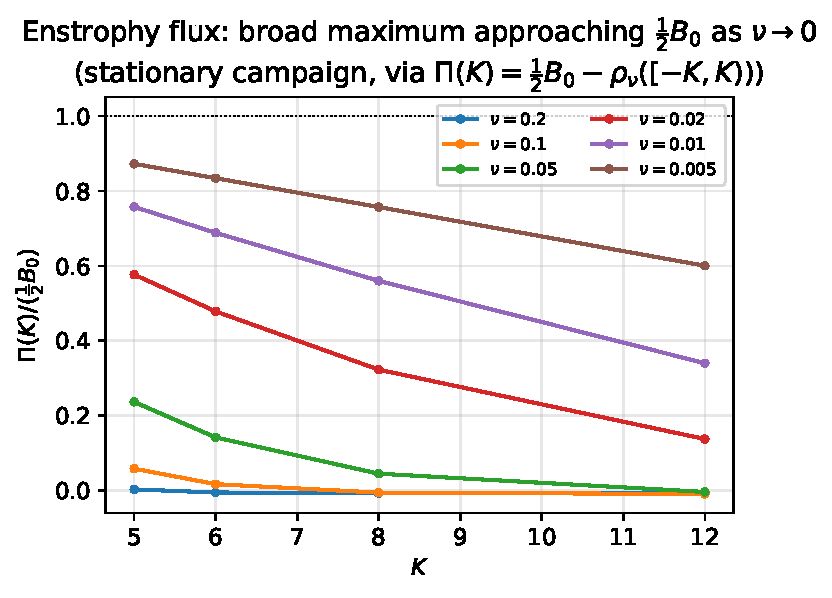
\includegraphics[width=0.62\textwidth]{flux_pi.pdf}
\caption{Enstrophy flux $\Pi(K)/(\tfrac12 B_0)$ from the stationarity-controlled campaign
(\S4), computed through the exact identity $\Pi(K) = \tfrac12 B_0 - \rho_\nu(\{|k|<K\})$
(Theorem A1, $K > k_f$): a broad maximum near $K=5$ that grows and approaches $\tfrac12 B_0$
as $\nu\to0$, then decays in the dissipation range. This is \emph{not} a resolved
inertial-range plateau (under one octave of scale separation between the forcing band
$[1,4]$ and the maximum). Statistical uncertainties (per-seed jackknife on $\rho_\nu$,
two seeds per point) are $\lesssim$ marker size; see Table~\ref{tab:campaign17}.
Data: \texttt{anc/p2\_results\_v18.jsonl}.}
\label{fig:flux}
\end{figure}

\emph{An earlier coarse exploratory sweep is retained only for the $a$-dependence
reported next; its recorded windows were not demonstrably at stationarity (split-half
$z$ up to $13$--$28$, Appendix~\ref{app:verification}), so we quote no error bars from it and have re-sourced every
quantitative flux and scaling statement above to the stationary campaign of \S4.}

\paragraph{Bridge to the deterministic blow-up literature (qualitative).} The coarse
$a$-sweep ($\nu=0.03$) shows the mean palinstrophy production \textbf{rising monotonically
as advection weakens} ($E[\mathcal{P}_1]$ roughly tripling from $a=-2$ to $a=-0.5$), with the
run \textbf{blowing up at $a=0$} (the CLM point, where finite-time singularity is expected).
Being drawn from the exploratory sweep, this is a qualitative trend --- we quote no
uncertainties. It is \emph{consistent with}, in the stationary stochastic setting,
the deterministic principle that stronger advection depletes stretching and
prevents singularity (Elgindi--Jeong \cite{ElgindiJeong2020}; Chen--Hou--Huang \cite{CHH2021}), and with the
forced-turbulence-vs-singularity study of the gCLM family by
Matsumoto--Sakajo \cite{MS2017} --- the $a=-2$ anomalous-
cascade state is the maximally advection-balanced member of the family. \emph{(The $a=0$
run is flagged under-resolved ($z=$nan, Appendix~\ref{app:verification}), so the blow-up there is consistent with
the singularity but not by itself evidence for it; the monotone trend at
$a\in[-2,-0.5]$ is the substantive observation.)}

\begin{thmA2}[Palinstrophy production balance]
For every invariant $\mu$ (Galerkin-rigorous; formal for (SG), \S2),
\begin{equation}
   \nu\, E_\mu\bigl[\textstyle\int\omega_{xx}^2\bigr] = E_\mu[\Pi_1] + \tfrac12 B_2, \qquad
   \Pi_1 = 2\int(H\omega)\omega_x^2 + \int(H\omega_x)\,\omega\,\omega_x,
\end{equation}
with the secondary term $\int(H\omega_x)\omega\omega_x = -\tfrac12\int(H\omega_{xx})\omega^2$.
\end{thmA2}

\emph{Proof: Appendix~\ref{app:identities} (C.3); certified to residual $10^{-15}$ (Appendix~\ref{app:verification}).}
Super-dissipation balances the nonlinear palinstrophy production plus injection
$\tfrac12 B_2$; $E_\mu[\Pi_1]$ is the mean nonlinear contribution to the palinstrophy
balance (its sign is not claimed a priori; measured positive, Appendix~\ref{app:verification}).

\section{The production balance and the normalized production diagnostic}

\paragraph{Role of $\mathcal{P}_1$ versus $\Pi_1$.} The full nonlinear term of the
palinstrophy balance (Theorem A2) is $\Pi_1 = 2\mathcal{P}_1 + \int(H\omega_x)\omega\omega_x$. The
production-balance analysis of this section applies the generator to $\mathcal{P}_1$
\emph{itself}: $\mathcal{P}_1$ is the functional we differentiate (the production
observable), whereas $\Pi_1$ is a term \emph{in} the balance \emph{of} the palinstrophy
$\mathcal{E}_1$ --- two distinct roles. We choose $\mathcal{P}_1$ rather than $\Pi_1$
because $2\mathcal{P}_1$ is the part of $\Pi_1$ whose own balance produces the
sign-definite term $W_1$ below; applying the generator to the secondary term
$\int(H\omega_x)\omega\omega_x$ yields no sign-definite leading term. This choice is part of the
grouping-dependence disclosed in \S5 (Normalization and interpretation).

\paragraph{The functional and its inertial balance (proved).} $\mathcal{P}_1 = \int(H\omega)\omega_x^2$,
$D\mathcal{P}_1 = -H(\omega_x^2) - 2(H\omega_x)\omega_x - 2(H\omega)\omega_{xx}$
(Lemma~\ref{lem:dp1}; certified against finite differences, Appendix~\ref{app:verification}). The inertial part
$I(a) = \langle b_{nl}, D\mathcal{P}_1\rangle$,
$b_{nl} = -au\omega_x + v\omega$, is (Proposition~\ref{prop:Ia}, proved for general fields in
Appendix~\ref{app:identities}; certified to machine precision, Appendix~\ref{app:verification}; $v=H\omega$,
$v_x=H\omega_x$, $u=-\Lambda^{-1}\omega$):
\begin{equation}
\begin{aligned}
   I(a) = {}& (2-2a)\int v^2\omega_x^2 - 2a\int uv\,\omega_x\omega_{xx} + 2\int v v_x\,\omega\omega_x \\
   & + a\int u\,\omega_x\, H(\omega_x^2) - \int v\,\omega\, H(\omega_x^2).
\end{aligned}
\end{equation}

At $a=-2$ the leading term is the \textbf{sign-definite} production-of-production
$W_1 \eqdef 6\int(H\omega)^2\omega_x^2 \ge 0$; the remainder $-N_1 \eqdef I - W_1$ is nonlocal (carries $u$ and
$H$; displayed explicitly in Appendix~\ref{app:identities}).

\paragraph{The projected balance (exact at every truncation).} On $E_M$ the generator
pairs the drift with the \emph{projected} gradient $P_M D\mathcal{P}_1$ --- and, unlike
the test functions of the \S3 balances, $D\mathcal{P}_1$ is quadratic and leaves $E_M$.
The exact nonlinear contribution of the Galerkin generator is therefore the projected
pairing
\begin{equation}
   I_M \eqdef \bigl\langle P_M N[\omega],\, P_M D\mathcal{P}_1\bigr\rangle
   \;=\; I - R_M, \qquad
   R_M \eqdef \bigl\langle Q_M N[\omega],\, Q_M D\mathcal{P}_1\bigr\rangle,\quad Q_M = \mathrm{Id} - P_M,
\end{equation}
and stationarity with Injection Lemma (injection $\equiv 0$) gives, \textbf{exactly at every
fixed truncation},
\begin{equation}\label{eq:pbexact}
   E_\mu[I_M] = -\mathcal{C}_1,
   \qquad\text{equivalently}\qquad
   E_\mu[N_1] = E_\mu[W_1] + \mathcal{C}_1 - E_\mu[R_M],
\end{equation}
with $\mathcal{C}_1 \eqdef \nu\, E_\mu[\langle \omega_{xx}, D\mathcal{P}_1\rangle]$
(no projection is needed in the viscous pairing: $\omega_{xx} \in E_M$), where
$\mathcal{C}_1$ is the \textbf{viscous contribution} (measured negative at the small-
and intermediate-$\nu$ operating points; at large $\nu$ the direct estimator is
SNR-limited, Appendix~\ref{app:verification}, and the sign is supplied by Theorem F for $M \ge 2k_f$; we
call it the viscous \emph{destruction} where hypothesis (NEG) of \S5 is in force).
The defect $R_M$ is structurally small:

\begin{lemma}[Support lemma for the Galerkin defect]\label{lem:rm}
If $\omega$ is supported on modes $|k| \le K$ with $2K \le M$, then $R_M(\omega) = 0$.
In particular, $E_G[R_M] = 0$ for the Ornstein--Uhlenbeck Gaussian of a forcing band
$k_f \le M/2$.
\end{lemma}

\emph{Proof.} $N[\omega]$ and $D\mathcal{P}_1(\omega)$ are quadratic in $\omega$, hence
supported on modes $|k| \le 2K \le M$; $Q_M$ annihilates both factors. $\qed$

\begin{remark}[The defect is not identically zero: $M=1$]\label{rem:m1}
For $\omega = A\cos x$ and $M = k_f = 1$: $N[\omega] = \tfrac32 A^2\sin 2x$ and
$D\mathcal{P}_1 = \tfrac52 A^2\sin 2x$ are pure second harmonics, so $P_1 N[\omega] = 0$
--- the one-mode Galerkin system is a \emph{linear} OU system with $I_M \equiv 0$ and
$\mathcal{C}_1 = 0$ --- while $I = \tfrac{15\pi}{4}A^4$ and $W_1 = \tfrac{9\pi}{2}A^4$,
so $I/W_1 = \tfrac56 \ne 0$. The full pairing $I$ is therefore \emph{not} the generator
contribution in general, and the two normalized objects below genuinely differ at small
$M$. (Certified in \texttt{anc/certify\_projected\_generator.py}, Appendix~\ref{app:verification}.)
\end{remark}

\paragraph{Two normalized objects.} We accordingly distinguish
\begin{equation}
   \theta \eqdef 1 - \frac{E_\mu[N_1]}{E_\mu[W_1]} = \frac{E_\mu[I]}{E_\mu[W_1]}
   \qquad\text{and}\qquad
   \theta_M \eqdef \frac{E_\mu[I_M]}{E_\mu[W_1]} = -\frac{\mathcal{C}_1}{E_\mu[W_1]},
\end{equation}
the \textbf{normalized production diagnostic} (grouping-dependent, scale-blind ---
Lemma~\ref{lem:scaleblind} --- and directly measurable: the object of all measured
curves and of Theorem F's first bound) and the \textbf{exact balance coefficient} of
the truncated system. By \eqref{eq:pbexact} they differ by the Galerkin defect,
$\theta - \theta_M = E_\mu[R_M]/E_\mu[W_1]$, which we measure at every operating point
(Table~\ref{tab:campaign17}): from $\sim10^{-8}$ at $\nu \ge 0.05$ through
$\approx 3\cdot10^{-5}$ at $\nu = 0.01$ to $\approx 5\cdot10^{-3}$ at $\nu = 0.005$,
where the spectrum fills toward the cutoff and $R_M$ becomes a genuine truncation
boundary term. The two objects respond differently to the cutoff: at $\nu = 0.005$ the defect drops
from $4.7\cdot10^{-3}$ ($M = 85$, pooled) to $5.3\cdot10^{-5}$ ($M = 127$) --- two orders of
magnitude for a $1.5\times$ cutoff increase --- while $\theta$ itself is unchanged
($0.7722$ at both cutoffs, within one band): $\theta$ is $M$-stable, while $\theta_M$ is the
balance coefficient \emph{of the particular truncated system}: in the two cutoff
checks performed, increasing $M$ reduced the positive normalized defect while $\theta$
stayed within one statistical band (we do not claim a proved sign or monotonicity of
$E_\mu[R_M]$ in $M$). This is why we report $\theta$ as the primary measured
object and $\theta_M$ alongside it. A genuine distinction of objects, not a convention.

\paragraph{Measured (proved-supported) --- the diagnostic is positive and
$\nu$-stable.} On the stationary state sampled by the solver at $a=-2$ (Appendix~\ref{app:verification};
2 seeds each; the campaign of Table~\ref{tab:campaign17} and
Figure~\ref{fig:theta}):
\begin{equation}
   \theta = 0.789\ (\nu=0.05), \quad 0.781\ (\nu=0.02), \quad 0.776\ (\nu=0.01).
\end{equation}

$\theta \in (0,1)$ --- two separate observations: $\mathcal{C}_1 < 0$ is measured,
which by the exact balance \eqref{eq:pbexact} gives $\theta_M > 0$; and
$E_\mu[I] > 0$, $E_\mu[N_1] > 0$ are measured, giving $0 < \theta < 1$ directly ---
and $\theta$
\textbf{decreases only gently across a decade of $\nu$, toward a finite positive limit} ---
empirical support for a floor $\theta \ge \theta_0 > 0$ (\S6). \emph{(The primary dataset
for Table~\ref{tab:campaign17} and Figure~\ref{fig:theta} is the exact-OU campaign
\texttt{anc/p2\_results\_v18.jsonl}, and the three values above are its pooled per-$\nu$
means. These are 2-seed points; the within-run $n=2$ standard error is uninformative and is
not quoted --- the per-seed jackknife band of Table~\ref{tab:campaign17} is $\pm0.0006$, and
the cross-code spread reported next is a separate, systematic scatter.)} An
\textbf{independent re-measurement on separately written code} (a plain Euler--Maruyama
solver, blind to the integrating-factor implementation; Appendix~\ref{app:verification}) gives
$\theta = 0.807, 0.771, 0.781, 0.775$ at
$\nu = 0.05, 0.02, 0.01, 0.005$, agreeing with the campaign to $\lesssim2.3\%$ (largest at
$\nu = 0.05$, where the two time-steppers' $O(dt)$ biases differ most), and shows $\theta$ \textbf{varying mildly within $[0.77, 0.81]$ across the small-$\nu$ range $\nu \in [0.005, 0.2]$} (Figure~\ref{fig:theta})
(the $\nu=0.01$ point fully resolved, dealiased tail $3\cdot10^{-11}\times$ peak); above
$\nu \approx 0.5$ it climbs to the Gaussian anchor $\theta_G \approx 0.812$ (\S4, large-$\nu$).
\emph{($\theta$ computed w.r.t.\ the leading square
$W_1 = 6\int v^2\omega_x^2$; an alternative admissible grouping $W_1' = c\,W_1$ rescales the value
($\theta' = \theta/c$, which for $c<1$ may exceed $1$) but preserves the qualitative sign
conclusion $\theta > 0$ and its $\nu$-stability. The two-sided bracket $\theta \in (0,1)$ is
reported for the stated $W_1$-grouping.)}

\paragraph{Stationarity-controlled campaign.} Long exact-OU-stepped runs (burn-in $\ge 5/\nu$, stationary windows
$\ge 20/\nu$, two seeds per point, block statistics; split-half drift $z$
reported \emph{on the observables themselves} --- $z \eqdef (\bar X_1 - \bar X_2)/\mathrm{SE}(\bar X_1 - \bar X_2)$,
the standardized difference of the first- and second-half block means of an observable $X$ over the
jackknife standard error of that difference, so $|z| < 2$ detects no statistically resolvable drift (a diagnostic, not a proof of stationarity) --- per-run controls: $L_0$ ratio
$\in [0.95, 1.06]$, dealiased tail $\le 9\cdot10^{-7}\times$ peak, hereditary-lemma
$\Pi_{LL} \sim 10^{-19}$; parameters in Table~\ref{tab:numerics}, Appendix~\ref{app:verification}):
\begin{table}[htbp]
\centering\small
\caption{The stationary campaign (strict-mask solver, padded diagnostics; two seeds per
point; pooled $\theta$ = ratio of the seeds' combined sample means, uncertainty =
per-seed block jackknife). $\theta - \theta_M = E[R_M]/E[W_1]$ = the normalized Galerkin
defect (\S4); $\delta_{\rm bal} = |E[I_M]+\mathcal{C}_1|/E[W_1]$ = the balance residual
(dominated by the statistical error of the noisy $\mathcal{C}_1$ estimator);
split-half $\max|z|$ over $I, W_1, \mathcal{E}_1, D$. Padded-vs-unpadded aliasing
receipts: $|\Delta\theta| \le 4\cdot10^{-6}$ at every point. ($R_M$ is measured
positive at every operating point, so the signed column $\theta-\theta_M$ and the
absolute defect $\delta_M$ of Appendix~\ref{app:verification} coincide.) Data:
\texttt{anc/p2\_results\_v18.jsonl}.}
\label{tab:campaign17}
\begin{tabular}{r|llllll}
$\nu$ & $\theta$ (pooled) & $\theta - \theta_M$ & $\delta_{\rm bal}$ & $\max|z|$ & $\rho_\nu(\{|k|<5\})/(\tfrac12 B_0)$ & HH share of $\Pi(5)$ \\
\hline
0.2   & $0.8061 \pm 0.0005$ & $<10^{-12}$ & $1.7\cdot10^{-2}$ & 1.6 & 0.997 & 0.005 \\
0.1   & $0.7978 \pm 0.0006$ & $<10^{-12}$ & $9\cdot10^{-3}$ & 1.5 & 0.941 & 0.023 \\
0.05   & $0.7890 \pm 0.0006$ & $2.3\cdot10^{-8}$ & $3.1\cdot10^{-3}$ & 1.2 & 0.763 & 0.064 \\
0.02   & $0.7808 \pm 0.0004$ & $1.4\cdot10^{-6}$ & $1.7\cdot10^{-3}$ & 1.7 & 0.424 & 0.139 \\
0.01   & $0.7758 \pm 0.0003$ & $3.3\cdot10^{-5}$ & $2.4\cdot10^{-3}$ & 0.6 & 0.243 & 0.194 \\
0.005   & $0.7722 \pm 0.0001$ & $4.7\cdot10^{-3}$ & $2.5\cdot10^{-3}$ & 0.9 & 0.128 & 0.231 \\
\hline
\end{tabular}
\end{table}

\begin{figure}[htbp]
\centering
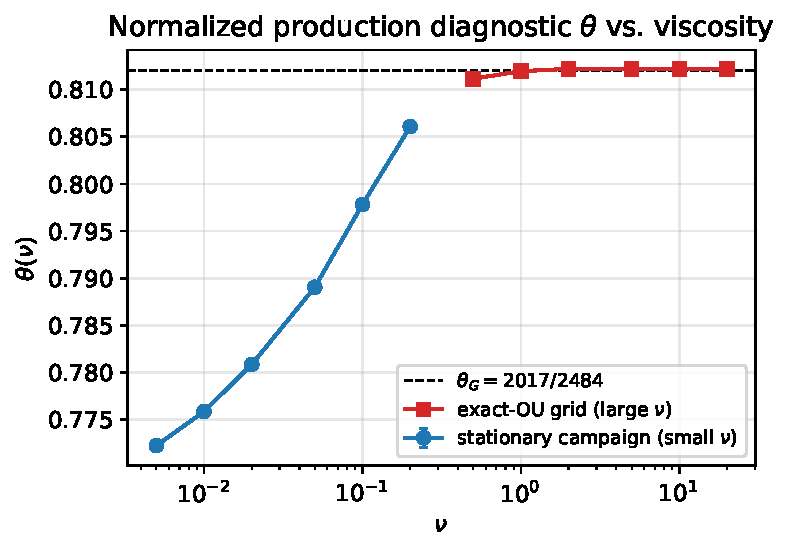
\includegraphics[width=0.62\textwidth]{theta_vs_nu.pdf}
\caption{The production-balance diagnostic $\theta(\nu)$: a small finite-$\nu$ deficit below the
Gaussian anchor $\theta_G = 2017/2484$ (stationary campaign, small $\nu$), climbing to $\theta_G$ by
$\nu\approx0.5$ (exact-OU grid, large $\nu$). Two seeds per point. Data:
\texttt{anc/p2\_results\_v18.jsonl}, \texttt{anc/theta\_large\_nu\_exact\_ou.log}.}
\label{fig:theta}
\end{figure}

\begin{figure}[htbp]
\centering
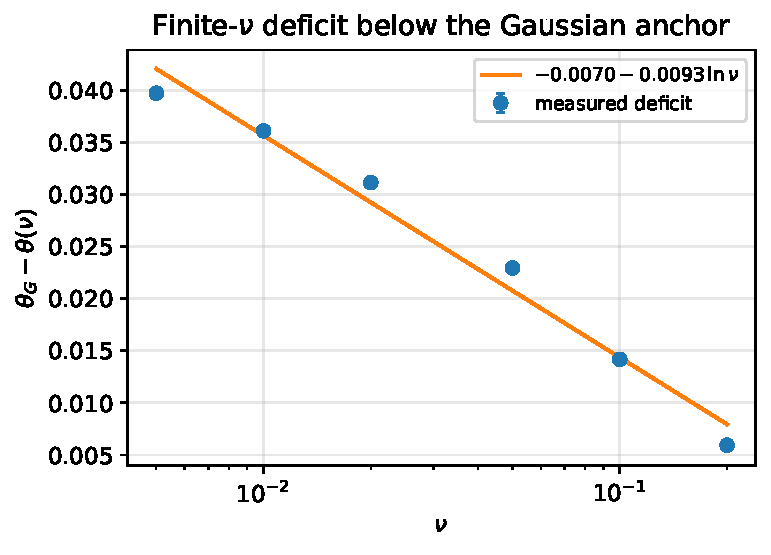
\includegraphics[width=0.48\textwidth]{theta_deficit.pdf}\hfill
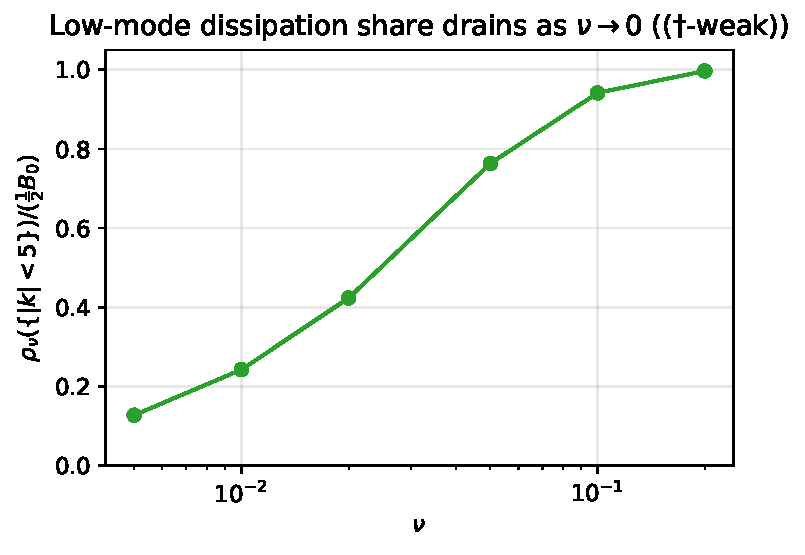
\includegraphics[width=0.48\textwidth]{rho_drain.pdf}
\caption{Left: the finite-$\nu$ deficit $\theta_G-\theta(\nu)$ is well described by a logarithm
$\approx -0.0070 - 0.0093\ln\nu$ over $\nu\in[0.005,0.2]$ (descriptive fit, no extrapolation
claimed). Right: the low-mode dissipation share $\rho_\nu(\{|k|<5\})/(\tfrac12 B_0)$ drains from
$\approx1$ to $0.128$ as $\nu\to0$ --- the empirical form of $(\dagger\text{-weak})$ with a rate.
Data: \texttt{anc/p2\_results\_v18.jsonl}.}
\label{fig:deficit}
\end{figure}

($dt/2$ check at $\nu=0.01$: $\theta = 0.7754 \pm 0.0003$, consistent; the full
step/resolution convergence matrix is reported in Appendix~\ref{app:verification}, Table~\ref{tab:convergence}.) Three
findings. (i) The finite-$\nu$ deficit below the exact Gaussian anchor
$\theta_G = 2017/2484$ is resolved and is well described by a \textbf{logarithm} over the
measured range (Figure~\ref{fig:deficit}): $\theta_G - \theta(\nu) \approx -0.0070 - 0.0093\ln\nu$ (coefficient s.e.\ $0.0025$,
$0.0007$; max residual $0.0025$, at the endpoint $\nu = 0.005$) --- a purely descriptive fit over the six points
$\nu \in [0.005, 0.2]$, asserting no functional form and claiming no extrapolation. (ii) The low-mode
dissipation share drains with an \emph{increasing} local rate: $\rho_\nu \sim
\nu^{\alpha_{\rm loc}}$ with $\alpha_{\rm loc} = 0.08 \to 0.30 \to 0.64 \to 0.80
\to 0.93$ between adjacent $\nu$ (propagated s.e.\ $\le 0.03$ per exponent). These
finite-difference exponents are sensitive to statistical and resolution error and are
reported as an empirical trend consistent with $(\dagger\text{-weak})$, not as evidence
of a limit $\alpha \to 1$. (iii) The negative inertial-generation fraction is $0$ on every
stationary sample ($n$ up to $8000$ per run): $I > 0$ pointwise along every
recorded trajectory.

\paragraph{The Gaussian anchor: $\theta_G$ is the large-$\nu$ limit.} Expand the Wick
(Gaussian) expectations $E_G[I]$ and $E_G[W_1]$ over the rescaled OU stationary shape in the
per-mode variances $s_k^2$: by independence only the diagonal ($s_k^4$) and cross
($s_i^2 s_j^2$) monomials survive, with coefficients $c_{\bullet,kk}$ and $c_{\bullet,ij}$
(the explicit Wick sums and the degenerate Gaussian $G_\nu = \mathcal{N}(0,\mathrm{diag}(b_k^2/(2\nu k^2)))$
they arise from are written out in Lemma~\ref{lem:appthetaG}, Appendix~\ref{app:thmF}).
The \textbf{cross-mode coefficient ratio}
\begin{equation}
   \theta_G(m) \eqdef c_{I,ij}/c_{W,ij} = (5+7m+3m^2)/(3+12m+3m^2), \qquad m = j/i\ (i<j),
\end{equation}
is the pairwise-interaction ratio of a single mode pair --- \emph{not} the ratio
$E_G[I]/E_G[W_1]$ of a two-mode field (certified, Appendix~\ref{app:verification}). It has global
minimum $\theta_{G,\min} = 1/3 + \sqrt{69}/18 \approx 0.7948$ at the non-integer
$m^* = (2+\sqrt{69})/5 \approx 2.06$ (minimality
independently re-verified, Appendix~\ref{app:verification}). (As a bare rational function $\theta_G(m)$
is \emph{not} bounded by $1$ --- it reaches $5/3$ as $m\to0$ and crosses $1$ at $m=2/5$; the
$\theta_G\in[\theta_{G,\min},1)$ range relies on the physical convention
$m=j/i>1$ ($i<j$), where $m^*=2.06$ is the interior minimizer.) The full-band value
$\theta_G(\text{band}) = E_G[I]/E_G[W_1]$ is the $c_W$-weighted mediant of the diagonal
self-ratio $c_{I,kk}/c_{W,kk} = 5/6$ and the cross ratios $\theta_G(j/i)$; since every weight
$c_{W,\bullet} > 0$ and every ratio is $\ge \theta_{G,\min}$ (verified for band $[1,4]$: the
minimum attained over its integer pairs is $\theta_G(2) = 31/39 = 0.7949$ at $m = 2$,
just above the family infimum $0.7948$ at the unattainable $m^* \approx 2.06$; diagonal
$5/6$), the band value provably exceeds the floor.
For the \emph{flat} (equal-amplitude) forcing band $[1,4]$ the
Gaussian value is the exact rational number $\theta_G(\text{flat band}) = 2017/2484 =
0.811996779\ldots$ (exact Wick sums in rational arithmetic; confirmed by direct sampling
of the Ornstein--Uhlenbeck stationary law to $5.6\cdot10^{-5}$; scripts in Appendix~\ref{app:verification}).
Because $\theta$ is a ratio of two quartic functionals (hence $0$-homogeneous in the field
amplitude) and the rescaled OU stationary shape $s_k^2 \propto b_k^2/k^2$ is
$\nu$-independent, $\theta_G(\text{band})$ is the \textbf{$\nu\to\infty$ limit of
$\theta$} (proved at the Galerkin level, Theorem F \S6; the solver evolves such a
system exactly in space, with the nonlinear drift advanced explicitly in time), and this is what the solver measures: with exact-OU noise stepping,
$\theta = 0.8111$--$0.8123$ (CI95 half-widths $\lesssim4\cdot10^{-4}$, split-half $z$ clean,
$dt/5$-stable) \emph{uniformly} across $\nu \in \{0.5, 1, 2, 5, 10, 20\}$, two seeds each.
The small-$\nu$ points ($0.772$--$0.789$ over $\nu \in [0.005, 0.05]$) thus read as a
\textbf{small finite-$\nu$ non-Gaussian deficit below the Gaussian anchor}, from which
$\theta(\nu)$ climbs back to $\theta_G$ by $\nu \approx 0.5$. The small-$\nu$ deficit is resolved by
the stationarity-controlled campaign below, reaching $\approx 0.040$ at $\nu = 0.005$.

\begin{lemB0}[Homogeneous-noise injection vanishes]
For homogeneous
noise $b_k=f(|k|)$, the It\^o injection into the palinstrophy production balance
vanishes: $\tfrac12\mathrm{Tr}(Q D^2\mathcal{P}_1) = 0$.
\end{lemB0}

\emph{Proof.} $D^2\mathcal{P}_1(h,h) = 2\int(H\omega)h_x^2 + 4\int(Hh)\omega_x h_x$. The
individual $\cos_k$ and $\sin_k$ trace summands do \emph{not} separately vanish; rather,
at the common homogeneous amplitude $b_k$ the two members of each $(\cos_k,\sin_k)$ pair
enter the trace with equal and opposite weight, so each $|k|$-pair cancels and the total
trace is $0$. Homogeneity is essential: with unequal amplitudes on the pair the trace is
genuinely nonzero (certified below). $\qed$

(Certified: homogeneous $10^{-16}$, anisotropic $\ne0$; Appendix~\ref{app:verification}.) Thus the
production balance \eqref{eq:pbexact} is injection-free:
$E_\mu[N_1] = E_\mu[W_1] + \mathcal{C}_1 - E_\mu[R_M]$, with no It\^o term.

\section{Reduction, conditional bound, density (corollaries of the production balance)}

Given the certified production balance of \S4, the following consequences are proved below;
all proofs are self-contained and rest only on the standing hypotheses (PB), (NEG),
(POS) stated next (each result names which of them it uses). These are corollaries of the
balance --- an algebraic reduction (Corollary~C) and a moment inequality (Corollary~E) ---
recorded to delimit what the diagnostic $\theta$ does and does not control; the paper's
main new theorem is the large-viscosity limit (Theorem~F, \S6).

\subsection*{Standing hypotheses}

\begin{itemize}
\item \textbf{(PB)} Production balance (exact at every truncation via the projected
  pairing, eq.~\eqref{eq:pbexact}): for every invariant $\mu$ of the Galerkin system,
  $E_\mu[I_M] = -\mathcal{C}_1$, i.e.\
  $E_\mu[N_1] = E_\mu[W_1] + \mathcal{C}_1 - E_\mu[R_M]$, where $W_1 \ge 0$ pointwise is
  the production-of-production, $N_1$ the nonlocal coherence term, and $R_M$ the
  measured Galerkin defect (Lemma~\ref{lem:rm}; per-point values in
  Table~\ref{tab:campaign17}, from $\sim10^{-8}$ to $\approx 5\cdot10^{-3}$ at the
  smallest $\nu$). The noise injection is
  \textbf{absent} (Injection Lemma: homogeneous-noise It\^o term $\equiv 0$, certified).
\item \textbf{(NEG)} $\mathcal{C}_1 \le 0$ (the mean viscous destruction is nonpositive).
  \emph{Status: a hypothesis, not a theorem} --- \S6 shows the sign of
  $\mathcal{C}_1 = \nu E_\mu[Y_{\rm d}]$ with $Y_{\rm d} \eqdef \langle\omega_{xx}, D\mathcal{P}_1\rangle$ exactly odd under $\omega\to-\omega$ is a property of the
  measure's asymmetry, not a pointwise inequality. It is \emph{measured} to hold cleanly at
  the small- and intermediate-$\nu$ operating points (\S4); at large $\nu$ the direct
  estimator is SNR-limited and the sign is \emph{not} statistically resolved there
  ($\nu = 10$: $\mathcal{C}_1 = -2.1\cdot10^{-4} \pm 2.7\cdot10^{-4}$) --- positivity of
  $\theta_M$ at large $\nu$ is a \emph{theorem} at the Galerkin level for $M \ge 2k_f$,
  with a strictly positive margin ($\theta_M \to \theta_G > 0$, Theorem F, \S6), though the
  theorem does not supply an explicit threshold $\nu_1$.
  Under (NEG), $E_\mu[N_1] \le E_\mu[W_1]$.
\item \textbf{(POS)} $E_\mu[W_1] > 0$ for every invariant measure. \emph{At a fixed
  Galerkin truncation this is a theorem, not a hypothesis} (Lemma~\ref{lem:pos}).
\end{itemize}

\begin{lemma}[Positivity of the production denominator]\label{lem:pos}
At a fixed Galerkin truncation, $E_\mu[W_1] > 0$ for every invariant measure $\mu$.
\end{lemma}

\emph{Proof.} $W_1 = 6\int(H\omega)^2\omega_x^2 = 6\|(H\omega)\,\omega_x\|^2 \ge 0$, so $W_1 = 0$
forces $(H\omega)\,\omega_x \equiv 0$. Since $H\omega$ and $\omega_x$ are real-analytic trigonometric
polynomials, the zero set of each is finite unless it vanishes identically; hence $H\omega \equiv 0$
or $\omega_x \equiv 0$, and either gives $\omega \equiv \text{const}$, so $\omega \equiv 0$ by zero
mean. Thus $W_1 = 0$ only at $\omega = 0$, and $E_\mu[W_1] = 0$ would force $\mu = \delta_0$; but
$\delta_0$ is not invariant under the nonzero additive noise ($B_0 > 0$). Hence $E_\mu[W_1] > 0$. $\qed$

\begin{definition}[Production diagnostic and balance coefficient]
\begin{equation}
\theta \eqdef 1 - \frac{E_\mu[N_1]}{E_\mu[W_1]} = \frac{E_\mu[I]}{E_\mu[W_1]},
\qquad
\theta_M \eqdef -\frac{\mathcal{C}_1}{E_\mu[W_1]} = \theta - \frac{E_\mu[R_M]}{E_\mu[W_1]}
\quad(\S4),
\end{equation}
well-defined real ratios under (POS); $\theta_M \ge 0$ iff (NEG) holds, and $\theta \le 1$
iff $E_\mu[N_1] \ge 0$ (a measured, not proved, sign). $\theta_M = 0$ exactly when the
destruction vanishes (steady/laminar trap); measured $\theta \in (0,1)$ at every operating
point with $\theta - \theta_M$ per point in Table~\ref{tab:campaign17} ($\le 0.7\%$ of
$\theta$ everywhere), and $\theta \to \theta_G(\text{shape})
\approx 0.812$ as $\nu\to\infty$ (\S4).
\end{definition}

\paragraph{Normalization and interpretation.} The ratio $\theta$ is defined
\emph{relative to the specific production grouping} $W_1 = 6\int(H\omega)^2\omega_x^2$ (the full,
sign-definite $\int v^2\omega_x^2$ term of $I$ at $a=-2$). This grouping is natural but not proved
canonical: a different admissible split $I = W_1' - N_1'$ rescales the denominator and hence the
numerical value of $\theta$; only the \emph{unnormalized} means $E_\mu[I]$ and
$E_\mu[I_M] = -\mathcal{C}_1$ are grouping-invariant. We therefore read $\theta$ as a \textbf{normalized, grouping-dependent
production-balance diagnostic}, not a canonical physical efficiency; the name ``cascade
efficiency'' of earlier versions is retired in favor of the neutral name. In particular (\S6, paragraph (S6)) a positive $\theta = O(1)$ is
compatible with the \emph{vanishing absolute-production limit} $E_\mu[W_1], |\mathcal{C}_1| \to 0$: $\theta$
measures the \emph{relative} balance of production against coherence, not the magnitude of an
absolute cascade. A canonical grouping (or a variational derivation of $W_1$) is open.

\begin{thmC}[Reduction]
Fix $\varepsilon \in (0,1)$. For any invariant $\mu$ (Galerkin-rigorous; formal for (SG), \S2;
assuming (POS), so that the
$\theta$-forms are well-defined),
\begin{equation}
   E_\mu[N_1] \le (1-\varepsilon) E_\mu[W_1]
   \quad\iff\quad \theta \ge \varepsilon
   \quad\iff\quad -\mathcal{C}_1 + E_\mu[R_M] \ge \varepsilon E_\mu[W_1],
\end{equation}
the last equivalence via the exact balance \eqref{eq:pbexact}; in terms of the balance
coefficient, $\theta_M \ge \varepsilon \iff -\mathcal{C}_1 \ge \varepsilon E_\mu[W_1]$.
A mean-coherence bound of margin $\varepsilon$ is EXACTLY a floor $\theta \ge \varepsilon$
on the diagnostic; up to the measured defect $E_\mu[R_M]$, a lower bound of
$\varepsilon E_\mu[W_1]$ on the viscous destruction $-\mathcal{C}_1$.
\end{thmC}

\emph{Proof.} The first equivalence is algebra ($I = W_1 - N_1$ pointwise, (POS)):
$E_\mu[N_1] \le (1-\varepsilon)E_\mu[W_1] \iff E_\mu[I] \ge \varepsilon E_\mu[W_1]
\iff \theta \ge \varepsilon$. The second substitutes
$E_\mu[I] = -\mathcal{C}_1 + E_\mu[R_M]$ from \eqref{eq:pbexact}. $\qed$

\textbf{Content.} $-\mathcal{C}_1$ is the \emph{viscous} destruction of the
palinstrophy production --- a purely dynamical object (it vanishes on the steady
trap) --- and $E_\mu[R_M]$ is the measured Galerkin defect ($\le 0.7\%$ relative at our
operating points, Table~\ref{tab:campaign17}). No kinematic/pointwise inequality can produce the margin: it lives in
the cascade dynamics. This localizes precisely what a proof of $\theta \ge \theta_0$ must supply.

\begin{remark}[Collapse of the conditional coherence bound]\label{rem:noD}
In a multi-component setting one would typically compare the coherence numerator $N$
against a \emph{separate} dissipation-comparable object $D$ ($W \ge D$,
$\beta \eqdef E[D]/E[W] \in (0,1]$), giving $R = E[N]/E[D] = (1-\theta)/\beta$ and a
margin $\varepsilon = 1 - (1-\theta_0)/\beta_{\min}$ under two floors $\theta \ge \theta_0$,
$\beta \ge \beta_{\min}$. In the 1D palinstrophy production balance \emph{as constructed
here} there is no independent
dissipation-comparable at the same order: the production-of-production $W_1$ and
the coherence $N_1$ are the only two $O(1)$ objects in the balance (Def $\theta$), the
destruction is $\mathcal{C}_1 = -E_\mu[I]$ (viscous), and no such $D_1$ arises
without introducing the palinstrophy-dissipation $\nu\int\omega_{xx}^2$, which lives at a
different order (the Level-1 balance, Theorem A2 of \S3). (This is an observation about
the term inventory of the present construction, not an impossibility theorem over a
defined class.) Consequently the conditional
coherence bound is \textbf{exactly Corollary C}: a floor $\theta \ge \theta_0$ gives, with no $\beta$
apparatus,
\begin{equation}
   E_\mu[N_1] \le (1 - \theta_0)\, E_\mu[W_1].
\end{equation}
\end{remark}

Measured (\S4, stationary campaign): $\theta \in [0.776, 0.789]$ across $\nu \in [0.01, 0.05]$, so
$E_\mu[N_1] \le 0.224 \cdot E_\mu[W_1]$ at the measured operating points --- the coherence is
comfortably sub-production. The 1D balance is \emph{cleaner} here (one fewer
hypothesis: no $\beta_{\min}$). \textbf{The genuinely open input is the $\theta_0 > 0$ floor},
which \S6 shows requires a \emph{scale-resolved} efficiency, not
this total-magnitude one.

\begin{thmE}[Density of negative inertial-generation episodes, moment form]
Define the \textbf{negative inertial-generation set} $\mathcal{A} \eqdef \{W_1 \le N_1\}$ --- states where the nonlocal
coherence overwhelms the local production-of-production ($\theta$ is locally negative).
Let $Y \eqdef W_1 - N_1 = I$ (pointwise), so $E_\mu[Y] = E_\mu[I] = \theta\cdot E_\mu[W_1]$
($= -\mathcal{C}_1 + E_\mu[R_M]$ by \eqref{eq:pbexact}).
Suppose (POS), $\theta > 0$ (measured at every operating point; a theorem at large $\nu$
for $M \ge 2k_f$, Theorem F), and $E_\mu[Y^2] < \infty$
(automatic at any fixed Galerkin truncation, Lemma~\ref{lem:appmoments}). Then
\begin{equation}
   \mu(\mathcal{A}) \;\le\; 1 - \frac{(E_\mu[Y])^2}{E_\mu[Y^2]}
   \;=\; 1 - \frac{\theta^2\,E_\mu[W_1]^2}{E_\mu[Y^2]} \;<\; 1,
\end{equation}
and, \emph{if $\mu$ is ergodic}, by Birkhoff's ergodic theorem the time-density of
negative inertial-generation episodes along $\mu$-typical trajectories obeys the same bound. For a
non-ergodic invariant $\mu$ the time-average along a typical trajectory equals the
conditional expectation $E_\mu[\mathbf{1}_{\mathcal{A}}\mid\mathcal{I}]$, so the bound
holds trajectory-wise only component-by-component (with each ergodic component's own
$\theta$, $E[W_1]$, $E[Y^2]$); the displayed bound then controls the $\mu$-average of these
densities. (At small $\nu$, where uniqueness/ergodicity is open, this distinction is
substantive and we do not elide it.)
\end{thmE}

\emph{Proof.} Under $\theta > 0$, $E_\mu[Y] = \theta E_\mu[W_1] > 0$. By Cauchy--Schwarz,
$E_\mu[Y] \le E_\mu[Y\mathbf{1}_{Y>0}] \le \sqrt{E_\mu[Y^2]\,\mu(Y>0)}$, hence
$\mu(Y>0) \ge (E_\mu[Y])^2/E_\mu[Y^2]$ and
$\mu(\mathcal{A}) = \mu(Y\le0) = 1 - \mu(Y>0) \le 1 - (E_\mu[Y])^2/E_\mu[Y^2]$.
Birkhoff applies since $\mathbf{1}_{\mathcal{A}}$ is bounded measurable. $\qed$

\begin{remark}[$L^\infty$ form]\label{rem:Linfty}
If additionally the excursion bound
$B \eqdef \operatorname*{ess\,sup}_\mu Y < \infty$ holds, with $b \eqdef B/E_\mu[W_1]$, then
$\mu(\mathcal{A}) \le 1 - \theta/b < 1$: for any r.v.\ with $Y \le B$,
$E[Y] = E[Y; Y\le0] + E[Y; Y>0] \le B\,\mu(Y>0)$, so
$\mu(Y\le0) \le 1 - \theta/b$ (non-vacuity $\theta \le b$ is automatic). However, with
additive Gaussian forcing the invariant measure is expected to have unbounded support on
the forced modes, so $B$ is plausibly \textbf{infinite} and is in any case not accessible
to finite simulation (a sample maximum estimates a quantile, never an essential
supremum): the $L^\infty$ form is a structural statement only, and Corollary E in its
moment form is the quantitative deliverable.
\end{remark}

\textbf{Reading.} A positive diagnostic $\theta$ forces the negative inertial-generation set to have
sub-unit measure. The inputs
are $\theta > 0$ (\S6) and a second moment of $Y$,
measurable at the operating points. Measured
(the \S4 stationary campaign, exact-OU-stepped, two seeds pooled per point; note
$Y = W_1 - N_1 = I$ pointwise): the bound gives $\mu(\mathcal{A}) \le 0.78$ at
$\nu = 0.05$ and $\le 0.80$ at $\nu = 0.01$ --- valid but far from tight: the
\emph{empirical} negative inertial-generation fraction is $0$ on every one of the
$8$k pooled stationary samples per point ($I > 0$ pointwise along the recorded trajectories;
the samples are time-correlated, so we report the observed fraction only and do
not convert it into a bound on $\mu(\mathcal{A})$). Given this large gap between the
loose bound ($\le0.78$) and the observed fraction ($0$), Corollary E is best
read as a \emph{qualitative} structural guarantee (a positive diagnostic forces the
negative inertial-generation set below full measure) rather than a sharp quantitative estimate.
The observed fraction $0$ on a finite, time-correlated sample is \emph{not} evidence that
$\{I\le0\}$ has zero measure, and does not establish kinematic positivity of $I$; whether
$I>0$ holds kinematically on band-limited fields is open, and would require a targeted search
(e.g.\ minimizing $I/W_1$ over band-limited fields) to decide.
(The quoted bounds are computed from the \S4 stationary campaign's padded
diagnostics, $E[Y^2]$ recorded per point.)

\subsection*{What is proved vs pending}

\begin{center}
\begin{tabular}{p{0.42\textwidth}p{0.50\textwidth}}
\hline
statement & status \\
\hline
Def $\theta$, $\theta_M$ (real ratios, under (POS)); (PB) exact via the projected pairing \eqref{eq:pbexact} & \textbf{proved} (Injection Lemma certified; Lemma~\ref{lem:rm} gives an exact support criterion for $R_M$'s vanishing and Lemma~\ref{lem:apprm} the large-$\nu$ bound; $\theta-\theta_M$ measured $\le 0.7\%$ of $\theta$, $\approx 5\cdot10^{-3}$ at the smallest $\nu$); canonical $W_1/N_1$ grouping open \\
$\theta \in [0,1]$, i.e.\ (NEG) $+$ $E_\mu[N_1]\ge0$ & \textbf{hypotheses}: measured at all operating points; (NEG) a theorem at large $\nu$, $M \ge 2k_f$ ($\theta_M\to\theta_G>0$, Thm F) \\
Cor C (reduction) & \textbf{proved} (algebra + \eqref{eq:pbexact}) \\
Remark~\ref{rem:noD} (conditional bound) & collapses to Cor C (no independent $D_1$ at this order in the present construction) \\
Cor E (negative inertial-generation density, moment form) & \textbf{proved} (given (POS), $\theta>0$; second moment automatic at Galerkin; ergodicity needed for the trajectory-wise reading) \\
the excursion bound $b < \infty$, uniform in $\nu$ & plausibly false ($B=\infty$); the $L^\infty$ form is Remark~\ref{rem:Linfty} only (measured moment bounds $0.78/0.80$; empirical negative inertial-generation fraction $0$) \\
$\theta \ge \theta_0 > 0$ uniformly in $\nu$ & OPEN at small $\nu$ (\S6); at large $\nu$ \textbf{proved at Galerkin level, $M \ge 2k_f$} (Thm F: $\theta, \theta_M \to \theta_G = 2017/2484$, so (NEG) is a theorem for $\nu \ge \nu_1$) \\
\hline
\end{tabular}
\end{center}

\section{The diagnostic floor: obstructions and the large-viscosity theorem}

We attacked $\theta \ge \theta_0 > 0$ and the flux-law input by four independent
strategies (verification record in Appendix~\ref{app:verification}). The honest outcome is \textbf{one new unconditional
theorem, a strict weakening of the open input, a certified structural lemma, and a
scale-blindness lemma} delimiting what the scalar $\theta$ can deliver --- not an
unconditional $\theta_0 > 0$, which meets a genuine turbulence-closure obstruction.

\paragraph{(S1) Unconditional --- flux law as UV-concentration (Corollary A1$''$, \S3).} The
two-hypothesis chain collapses to a hypothesis-free equivalence: $(\mathrm{FL}\infty) \iff \rho_\nu$
UV-concentrates. This \emph{replaces} the earlier over-hypothesized corollary.

\paragraph{(S2) Weakening --- $(\dagger) \to (\dagger\text{-weak})$.} The open input is $E_\mu\|P_{<K}\omega\|^2 = o(1/\nu)$,
not $O(1)$; the naive Poincar\'e bound sits exactly at the borderline exponent, so
only an $o(1)$ gain is needed.

\paragraph{(S3) Certified structural lemma --- hereditary advective cancellation.} The $a=-2$
cancellation is not a full-field accident: the low-mode Galerkin self-interaction
vanishes for \emph{every} truncation, $\langle \omega_L, P_{<K}N[\omega_L]\rangle \equiv 0\ \forall K$
(certified 24/24 to $\le 9\cdot10^{-14}$, Appendix~\ref{app:verification}). \emph{(It is a one-line
corollary of the A0 cancellation applied to $\omega_L$ via the self-adjoint idempotent
$P_{<K}$; the value is the decomposition it enables, not the proof depth.)} Hence
the flux $\Pi(K)$ is carried entirely by cross/high-mode leakage (a linear-in-$\|\omega_H\|$
term plus a quadratic one), which localizes what any proof of $(\dagger\text{-weak})$ must
control.

\paragraph{(S4) The scale-blindness obstruction --- why $\theta$ is not the bridge.}
The obstruction is now a lemma. For $\lambda \in \mathbb{N}$ let $S_\lambda$ denote the
\emph{mode dilation} $(S_\lambda\omega)(x) = \omega(\lambda x)$, i.e.\
$\widehat{S_\lambda\omega}(\lambda k) = \hat\omega(k)$ (and $=0$ off $\lambda\mathbb{Z}$).

\begin{lemma}[Scale-blindness of $\theta$]\label{lem:scaleblind}
$S_\lambda$ commutes with $H$ and with pointwise products, and satisfies
$\partial_x S_\lambda = \lambda\, S_\lambda \partial_x$ and
$\Lambda^{-1} S_\lambda = \lambda^{-1} S_\lambda \Lambda^{-1}$. Consequently every monomial
of $I$ and of $W_1$ is homogeneous of total dilation weight $2$, so for every field
\begin{equation}
   I(S_\lambda\omega) = \lambda^2\, I(\omega), \qquad W_1(S_\lambda\omega) = \lambda^2\, W_1(\omega).
\end{equation}
Hence for every probability measure $\mu$ on field space (finite fourth moments,
$E_\mu[W_1]>0$) and its dilation pushforward $\mu_\lambda \eqdef (S_\lambda)_*\mu$:
\begin{equation}
   \theta(\mu_\lambda) = \frac{E_{\mu_\lambda}[I]}{E_{\mu_\lambda}[W_1]}
   = \frac{\lambda^2 E_\mu[I]}{\lambda^2 E_\mu[W_1]} = \theta(\mu) \qquad \text{for every } \lambda,
\end{equation}
while the low-mode dissipation share is \emph{not} dilation-invariant: if $\mu$ is
supported on modes $|k| \le K_0 < K$, the share
$\rho_{\mu_\lambda}([-K,K))/\rho_{\mu_\lambda}(\mathbb{Z}^*)$ equals $1$ at $\lambda = 1$
and $0$ for every $\lambda > K$.
\end{lemma}

\emph{Proof.} On Fourier coefficients $S_\lambda$ relabels $k \mapsto \lambda k$: the $H$
multiplier $-i\,\mathrm{sgn}(\lambda k) = -i\,\mathrm{sgn}(k)$ ($\lambda>0$) commutes with the
relabeling (weight $0$); each $\partial_x$ contributes one factor $\lambda$ (weight $1$);
$\Lambda^{-1}$ contributes $1/|\lambda k| = \lambda^{-1}/|k|$ (weight $-1$); products are
pointwise, and $\int_0^{2\pi} f(\lambda x)\,dx = \int_0^{2\pi} f$ for $\lambda\in\mathbb{N}$.
Assigning weights $\omega \mapsto 0$, $v = H\omega \mapsto 0$, $u = -\Lambda^{-1}\omega \mapsto -1$,
each derivative $\mapsto +1$: every monomial of
$I = (2-2a)\!\int\! v^2\omega_x^2 - 2a\!\int\! uv\,\omega_x\omega_{xx} + 2\!\int\! v v_x\omega\omega_x
+ a\!\int\! u\omega_x H(\omega_x^2) - \!\int\! v\omega H(\omega_x^2)$ and of
$W_1 = 6\int v^2\omega_x^2$ has total weight $2$ ($0{+}0{+}1{+}1$; $-1{+}0{+}1{+}2$;
$0{+}1{+}0{+}1$; $-1{+}1{+}2$; $0{+}0{+}2$). The dissipation statement is immediate:
$\rho_{\mu_\lambda}$ carries its mass on modes $\lambda|k| \ge \lambda$. $\qed$

\begin{corollary}[No bound factoring through $\theta$ closes $(\dagger\text{-weak})$]\label{cor:noftheta}
There is no function $f$ with
$\rho_\mu([-K,K))/\rho_\mu(\mathbb{Z}^*) \le f(\theta(\mu)) < 1$ valid over all
probability measures: the Ornstein--Uhlenbeck Gaussian $G$ on the band $[1,2]$ has
$\theta(G) \ge \theta_{G,\min} \approx 0.7948$ (the mediant argument of \S4) and low-mode
share $1$ for $K > 2$, while its dilations $G_\lambda$ have the \emph{same} $\theta$ and
share $0$ for $\lambda > K$. Consequently any proof of $(\dagger\text{-weak})$ from a
floor $\theta \ge \theta_0$ must use the dynamical input that $\mu$ is an
\emph{invariant measure} of (SG) --- information not contained in the value of
$\theta$. In this precise sense $\theta$ is scale-blind: bounds factoring through the
scalar $\theta$ alone cannot control spectral localization.
\end{corollary}

\emph{Scope.} Lemma~\ref{lem:scaleblind} and its corollary concern the \textbf{full
diagnostic} $\theta = E[I]/E[W_1]$ ($I$, $W_1$ are functionals of the field alone,
and the dilation argument never invokes a balance). The exact balance coefficient
$\theta_M$ (\S4) carries the projector $P_M$, which does \emph{not} commute with
$S_\lambda$; a dilation statement for $\theta_M$ would compare \emph{different}
truncated systems, $(\omega, M) \mapsto (S_\lambda\omega, \lambda M)$, and we do not
claim it. Since the measured defect $\theta - \theta_M$ is $\le 0.7\%$ of $\theta$ at
every operating point (Table~\ref{tab:campaign17}), the obstruction reading is
unaffected.

\emph{Discussion (the mechanism behind Lemma~\ref{lem:scaleblind}).} Three complementary
routes anticipate the lemma
(locality mismatch: $W_1=6\int v^2\omega_x^2$ is an all-scales, $H$-unimodular functional
carrying no low-$k$ weight; dimensional: a dimensionless $\theta$ cannot convert the
$\nu^{-1}$-divergent Poincar\'e bound into $o(\nu^{-1})$; derivational: no
generator/Cauchy--Schwarz identity bridges the bilinear low-pass pairing to the
cubic unfiltered ratio). The precise missing ingredient is a
\textbf{scale-resolved efficiency} (a $K$-dependent floor on the rate at which
$\rho_\nu(\{|k|<K\})$ is driven to $o(1/\nu)$) plus a dynamical (martingale/Gr\"onwall)
argument. This is a genuine turbulence-closure obstruction: the total-magnitude
diagnostic is bounded and measured ($\theta \approx 0.78$, \S4), but the \emph{scale-resolved}
residual that the flux law actually needs is not controlled by it. (Honest scope:
Corollary~\ref{cor:noftheta} rules out bounds factoring through $\theta$ over the class
of all measures; it does not exclude dynamical arguments that use invariance itself.)

A \textbf{further obstruction route} (independent of the above) operates at
the level of $\theta$'s own integrand: the destruction integrand $Y_{\rm d} \eqdef \langle\omega_{xx}, D\mathcal{P}_1\rangle$ (an odd cubic --- distinct from Corollary E's even quartic $Y = W_1 - N_1$) is
\textbf{exactly odd under $\omega \to -\omega$} (machine-zero check, Appendix~\ref{app:verification}) and
pointwise sign-indefinite (Appendix~\ref{app:verification}) --- so $-E_\mu[Y_{\rm d}] > 0$
(hence $\theta_M > 0$; the diagnostic $\theta$ then differs by the measured defect) is a
property of the \emph{measure's} $\omega\to-\omega$-asymmetry, not a kinematic
inequality; no pointwise bound delivers it.

\paragraph{(S5) The measured evidence (\S4).} $\theta \approx 0.78$, $\nu$-stable across
the factor-$40$ range $\nu \in [0.005, 0.2]$ and $\theta \to \theta_G \approx 0.812$ at large $\nu$ ---
the diagnostic floor $\theta_0 > 0$ is empirically robust, but \emph{proving} it remains open
(\S6, the paper's central open problem); closing $(\mathrm{FL}\infty)$ additionally requires the
\emph{scale-resolved} input $(\dagger\text{-weak})$, not merely a total-magnitude floor. A
previously proposed positive mechanism --- a phase-homogeneity hypothesis
$(\star)$: $E_\mu[\Pi_{HH}] = 0$, i.e.\ the mean high--high flux piece (\S2) vanishes, which
would remove the small-scale leakage into the low-mode dissipation and reduce
$(\dagger\text{-weak})$ by one order --- is now \textbf{refuted as a small-$\nu$ mechanism}
(pre-registered falsifier): in the stationary campaign the mean HH (quadratic-in-$\omega_H$)
share of the flux $\Pi(5)$ \emph{grows monotonically} as $\nu$ decreases
(from $0.5\%$ at $\nu=0.2$ to $23.1\%$ at $\nu=0.005$), i.e.\ the
$(\star)$-consequence degrades exactly where the mechanism would be needed. The
same measurements give $(\dagger\text{-weak})$ \emph{with a rate}: the low-mode
dissipation share $\rho_\nu(\{|k|<5\})/(\tfrac12 B_0)$ drains from $1.0$ to $0.128$
over $\nu \in [0.2, 0.005]$ with local decay exponents $\alpha_{\rm loc}$
($\rho_\nu \sim \nu^{\alpha}$) rising $0.08 \to 0.93$ --- consistent with an
approach to $\alpha = 1$, which would amount to the \emph{original} uniform bound
$(\dagger)$, not just $(\dagger\text{-weak})$ (measured trend, not a claim).

\paragraph{(S6) Large $\nu$: a vanishing absolute-production limit with positive limiting
diagnostic.} The key point is that $\theta$ is a ratio of two \emph{quartic} functionals, hence $0$-homogeneous in
the field amplitude, and the rescaled OU stationary shape is $\nu$-independent; writing
$s^2 \sim B_0/\nu$ for the per-mode variance and $\varepsilon \sim s/\nu \sim \nu^{-3/2}$
for the effective coupling, the numerator $-\mathcal{C}_1 = -\nu E_\mu[Y_{\rm d}]$ has leading
order $\nu\cdot s^3\varepsilon = s^4$ --- the \emph{same} order as $E_\mu[W_1]$ ($Y_{\rm d}$ is
Gaussian-odd, so its first-order term carries $\varepsilon$, but the $\nu$ prefactor in
$\mathcal{C}_1$ exactly restores the balance). Hence
\begin{equation}
   \theta(\nu) \;\xrightarrow[\nu\to\infty]{}\; \theta_G(\text{shape}) \;\ge\; \theta_{G,\min} \approx 0.7948,
   \qquad\text{while}\qquad E_\mu[W_1],\ |\mathcal{C}_1| = O\!\bigl((B_0/\nu)^2\bigr) \to 0:
\end{equation}
\textbf{large viscosity is a vanishing absolute-production limit ($E[W_1]$ and the destruction both $\to 0$), not a diagnostic-null limit.}
Measured (exact-OU noise stepping, Appendix~\ref{app:verification}):
$\theta = 0.8111$--$0.8123$ uniformly over $\nu \in \{0.5,\dots,20\}$, matching
$\theta_G(\text{band}) = 0.8119 \pm 10^{-4}$; the direct-$\mathcal{C}_1$ route is an unreliable
estimator here, with signal-to-noise
$\sim \mathrm{mean}(Y_{\rm d})/\mathrm{rms}(Y_{\rm d}) \sim \varepsilon \approx 10^{-2}$ at $\nu=10$
(measured mean/rms $\approx 1/90$; the estimator's signal $4.4\cdot10^{-5}$ vs block-SE
$1.6\cdot10^{-4}$, Appendix~\ref{app:verification}). Consequently the
direct stationarity closure $E_\mu[I] = -\mathcal{C}_1$ is corroborated only to $\approx5\%$
at large $\nu$ ($\theta$ via the low-variance $E_\mu[I]$ estimator is $0.812$ vs $\theta$ via
$-\mathcal{C}_1$ is $0.856$ at $\nu=2$, $z(\mathrm{diff})=-0.54$); we therefore report $\theta$
through $E_\mu[I]$ (independently corroborated by a plain Euler--Maruyama solver at $0.81216$),
not the noisy $-\mathcal{C}_1$ route. The parity facts
themselves stand ($N[\omega]$ even, $Y_{\rm d}$ odd, $E_G[Y_{\rm d}]=0$): they say the \emph{absolute}
asymmetry vanishes as $O(\varepsilon)$, not that the ratio $\theta$ does. The outlook
consequently \emph{flips}: the FFS uniqueness/mixing regime is exactly where $\theta$ has
a positive Gaussian limit, so \textbf{a rigorous perturbative proof of
$\theta(\nu) \to \theta_G > 0$ at large $\nu$ --- positivity of the production
diagnostic in the rigorous regime --- is a concrete open target} (Poisson-equation/Wick
computation about the OU measure), whereas the uniform small-$\nu$ floor remains the
genuine closure obstruction. At the \emph{Galerkin} level this target is now met:

\begin{thmF}[Large-$\nu$ limit of the diagnostic, Galerkin level]
Fix a Galerkin cutoff $M \ge k_f$ and consider the spectral Galerkin system
$d\omega = (P_M N[P_M\omega] + \nu\omega_{xx})\,dt + dW$ on the mean-zero modes
$1 \le |k| \le M$, with homogeneous band noise, $B_0 = \mathrm{Tr}\,Q > 0$. There
are $C = C(M,\text{shape})$ and $\nu_0$ such that \emph{every} invariant measure
$\mu_\nu$ (no uniqueness assumed) satisfies, for $\nu \ge \nu_0$,
\begin{equation}
   \bigl|\,\theta(\mu_\nu) - \theta_G\,\bigr| \;\le\; C\,\sqrt{B_0}\;\nu^{-3/2},
\end{equation}
where $\theta_G = E_G[I]/E_G[W_1]$ on the Gaussian OU law of the forcing shape. If
moreover $M \ge 2k_f$, the same bound holds for the exact balance coefficient,
\begin{equation}
   \bigl|\,\theta_M(\mu_\nu) - \theta_G\,\bigr| \;\le\; C\,\sqrt{B_0}\;\nu^{-3/2}
   \qquad (M \ge 2k_f),
\end{equation}
because $E_G[R_M] = 0$ (Lemma~\ref{lem:rm}) and $E_{\mu_\nu}[R_M]$ obeys the same
quintic correction bound (Lemma~\ref{lem:apprm}). In particular $\mathcal{C}_1 < 0$
--- hypothesis (NEG), hence $\theta_M > 0$ ---
\textbf{holds as a theorem} for all $\nu \ge \nu_1(M, B_0, \text{shape})$ and $M \ge 2k_f$: to our
knowledge, the first proved positivity of this (grouping-dependent) balance
coefficient for the stochastic gCLM at $a=-2$, at the Galerkin level and for the stated
$W_1$-grouping. For the flat band $[1,4]$ the limit is, relative to the
$W_1$-grouping of \S5, the exact rational number
\begin{equation}
   \theta_G(\text{band}\,[1,4]) \;=\; \frac{2017}{2484} \;=\; 0.811996779\ldots
\end{equation}
\end{thmF}

\emph{Proof} (full argument in Appendix~\ref{app:thmF}; the exact constant is
independently certified, Appendix~\ref{app:verification}). \emph{Sketch.} (i) \emph{Moments:} by the
hereditary $a=-2$ cancellation $\langle P_MN[P_M\omega],\omega\rangle = 0$ (S3),
$V = \|\omega\|^2$ satisfies $\mathcal{L}V \le -2\nu V + B_0$ and
$\Gamma(V) \le 4B_0V$, giving $E_\mu[V^p] \le (2p-1)!!\,(B_0/2\nu)^p$ for every
invariant $\mu$ (concave-cutoff localization; this also justifies
$E_\mu[\mathcal{L}F]=0$ for every polynomial $F$ at the Galerkin level).
(ii) \emph{Poisson equation:} the OU generator is diagonal-plus-nilpotent on
polynomials, so $\varphi_F = \sum_j(-D^{-1}T)^jD^{-1}\tilde F$ is explicit, with a
$\nu^{-1}$ gain. (iii) \emph{Exact correction identity:}
$E_\mu[F] - E_G[F] = -E_\mu[\langle N_M, D\varphi_{\tilde F}\rangle]$, a quintic
bounded by $C\nu^{-1}s^5$ ($s^2 = B_0/2\nu$), against $E_G[W_1] = c_Ws^4$,
$c_W>0$. The solver evolves this Galerkin system exactly in space (drift and state projected to $E_M$; first-order in time), so the \S4
measurements ($\theta$ point estimates $0.8111$--$0.8123$, CI95-inclusive
$[0.8107,0.8126]$, over $\nu \in [0.5,20]$ vs
$\theta_G = 0.81200$) are consistent with the Gaussian limit predicted by Theorem~F. \emph{Honest
scope: the constant $C(M)$ grows with the cutoff; the untruncated (SPDE)
statement needs uniform-in-$M$ moments and Galerkin convergence of invariant
measures, both open. Small $\nu$ is untouched: the closure obstruction stands. (The
``every invariant measure, no uniqueness assumed'' formulation is a structural feature of
the proof, not a claim that non-uniqueness occurs at $\nu\ge\nu_0$: the Galerkin
system is expected uniquely ergodic there, and it is the small-$\nu$ identities of
\S3--\S5, where uniqueness is genuinely open, that the uniqueness-free formulation
protects.)}

\section*{Code and data availability}

All algebraic certifications and numerical measurements reported here are reproducible
from an accompanying code repository, organized as follows.
\begin{itemize}
\item \textbf{Solver.} A pseudo-spectral (Fourier) discretization of (SG) with
  Euler--Maruyama time stepping and $2/3$-dealiasing (\texttt{anc/}); validated
  on 12 independent identities (Verification ledger, Appendix~\ref{app:verification}).
\item \textbf{Symbolic certifications} of every algebraic identity (A0, A1, A1$''$, A2,
  the inertial formula $I(a)$, and the Injection Lemma), band-limited-spectral with
  residual $\equiv 0$ to machine precision (\texttt{anc/}).
\item \textbf{Measurement scripts} producing the stationary-measure estimates of the
  enstrophy balance, the anomalous-cascade exponent, the broad flux maximum, and the
  production diagnostic $\theta$, including the independent re-measurement of
  \S4 on separately written code and the convergence matrix
  (\texttt{anc/}, \texttt{anc/}).
\item \textbf{Obstruction analyses} for $(\dagger\text{-weak})$ and $\theta \ge \theta_0 > 0$:
  the hereditary-cancellation certification, the flux-sign and parity obstruction
  checks, and the large-$\nu$ limit measurements with exact-OU noise stepping and
  the stationary-balance closure check (\texttt{anc/}, in particular
  \texttt{theta\_large\_nu\_exact\_ou.py} and \texttt{closure\_balance\_check.py}).
\end{itemize}
The repository is public at \url{https://github.com/rifmj/sgclm-cascade}; \textbf{the
results of this version correspond to the tagged release \texttt{v1.14}}, archived at Zenodo,
\href{https://doi.org/10.5281/zenodo.21492681}{\texttt{doi:10.5281/zenodo.21492681}}. The
paper source is under \texttt{paper/} and the verification package (the CAS certificates, the
solver, and the single-command \texttt{make verify}) under \texttt{anc/}; see \texttt{anc/README.md}.
The model and its
large-viscosity ergodic theory are due to Fujita--Fukuizumi--Sakajo (arXiv:2603.06182).

\section*{Acknowledgements}

We are grateful to the anonymous referees of earlier versions of this paper for a
sequence of substantive improvements. In particular, the projected-pairing correction of
\S4 --- the distinction between the full inertial functional $I$ and the Galerkin
generator's contribution $I_M$, with the one-mode example of Remark~\ref{rem:m1} --- was
prompted by a referee's report, as were the scale-blindness lemma, the convergence
matrix, and the analytic proofs of Appendix~\ref{app:identities}.

\paragraph{Use of AI assistance.} The construction and write-up of this paper were
carried out with substantial assistance from AI tools, including for the exploratory
derivations and for the multi-round internal referee process. All mathematical claims
rest on the machine-checkable certificates (band-limited spectral certification, residuals
$10^{-14}$--$10^{-19}$) and the reproducible solver ($12/12$ self-test) documented above,
not on trust in those tools. The author has verified the results and is solely accountable
for them.

\appendix
\section{Verification: certificates, solver, and reproducibility}\label{app:verification}

\begin{table}[htbp]
\centering\small
\caption{Trusted-computing-base map: stage $\to$ program $\to$ arithmetic model $\to$
certified output. Primary inputs are the committed campaign data
(\texttt{anc/*.jsonl}); the tables and figures are derived outputs.}
\label{tab:tcb}
\begin{tabular}{p{0.26\textwidth} p{0.30\textwidth} p{0.18\textwidth} p{0.18\textwidth}}
\hline
stage & program & arithmetic & certified output \\
\hline
identities (A0--A2, $D\mathcal{P}_1$, $I(a)$, B0), symbolic & \texttt{anc/certify\_identities\_symbolic.py} & exact $\mathbb{Q}[a]$ & zero polynomials, $K \le 8$ \\
identities, spectral & \texttt{anc/certify\_*.py}, \texttt{anc/validate.py} & float64 & residuals $\le 10^{-14}$ \\
projected generator & \texttt{anc/certify\_projected\_generator.py} & exact rationals + float64 & $I = I_M + R_M$; support lemma; $M{=}1$ \\
$\theta_G$, exact & \texttt{anc/certify\_theta\_G\_exact.py} & exact rational Wick sums & $2017/2484$ (+ float MC cross-check) \\
stationary campaign & \texttt{anc/p2\_campaign\_v18.py} & float64; padded $L=2N$ diagnostics & Table~\ref{tab:campaign17} + receipts \\
convergence matrix & \texttt{anc/p2\_convergence\_matrix.py} + campaign receipts & float64; unpadded ($\le 4\cdot10^{-6}$) & Table~\ref{tab:convergence} \\
analysis / fits & \texttt{anc/p2\_analysis.py} & float64 & deficit log-law, $\alpha_{\rm loc}$, shares \\
\hline
\end{tabular}
\end{table}

\paragraph{Numerical method and error control (scope).} The solver is a pseudo-spectral (Fourier)
Galerkin truncation on $E_M$ with the \textbf{strict} $2/3$ rule $M = \lfloor (N-1)/3\rfloor$
($3M \le N-1$, so no product of retained modes aliases onto a retained mode --- with the
non-strict $\lfloor N/3\rfloor$ cutoff at $3 \mid N$ the boundary pair's self-product $2M$
aliases on the grid exactly onto the retained mode $-M$): the mask is applied to every factor
entering the quadratic products \emph{and} to the nonlinear result and the state, so the evolved
system is the Galerkin system on $E_M$ exactly (the state carries no energy above $M$).
The diagnostic functionals $I$, $I_M$, $R_M$, $W_1$, $\langle\omega_{xx}, D\mathcal{P}_1\rangle$
are evaluated on a \textbf{zero-padded} grid $L = 2N$ ($L/2 > 2M$ and $L > 4M$), so the
quadratic fields $N[\omega]$, $D\mathcal{P}_1$ and the quartic quadratures are exact,
alias-free evaluations of the paper's functionals; each campaign point also records the
unpadded pseudo-spectral values as an aliasing receipt (Table~\ref{tab:campaign17}).
(The dedicated convergence-matrix driver behind Table~\ref{tab:convergence} evaluates
$\theta$ through the unpadded $N$-grid path; the recorded aliasing impact on $\theta$
is $\le 4\cdot10^{-6}$, far below the statistical bands, so the matrix comparisons are
unaffected; its $N{=}384$ and $dt/2$ ($\nu=0.01$) rows are padded receipts from the
campaign pipeline.) Time stepping uses an
integrating-factor scheme in which
the viscous part and the additive-noise increment are advanced
\emph{exactly} in the linear variable (exact Ornstein--Uhlenbeck noise stepping, in
all runs), while the nonlinear drift is advanced by an explicit
first-order step; the scheme is therefore \emph{exact in space} but
\emph{first-order in time}. Alongside each campaign point we record the two dimensionless
diagnostics of the production balance: $\delta_M = |E[R_M]|/E[W_1]$ (the spatial-projection
defect separating $\theta$ from $\theta_M$, \S4; the campaign table's $\theta-\theta_M$
column) and
$\delta_{\rm bal} = |E[I_M] + \mathcal{C}_1|/E[W_1]$ (the residual of the exact balance
\eqref{eq:pbexact} in the time-discretized chain; dominated by the statistical error of the
noisy $\mathcal{C}_1$ estimator: $1.7\cdot10^{-3}$--$1.7\cdot10^{-2}$ across the small-$\nu$
campaign, and unusable at large $\nu$ where the estimator's SNR collapses ---
$\delta_{\rm bal} \approx 3$ at $\nu = 10$). (The tables' $\theta_M$ is computed through
the exact balance from the projected pairing $I_M$; the direct $-\mathcal{C}_1/E[W_1]$
estimator differs from it by up to $\delta_{\rm bal}$.) Reported values are stationary block averages; ratio uncertainties are
leave-one-block-out (block-jackknife) errors; split-half drift diagnostics
($z<2$ on the observables). Controls: dealiased
spectral-tail suppression ($\le 9\cdot10^{-7}\times$ peak), the hereditary-lemma check
$\Pi_{LL}\sim10^{-19}$, and the convergence matrix of Table~\ref{tab:convergence}
(plotted in Figure~\ref{fig:convergence}). The
quoted $\pm$ bands are conditional statistical (block-bootstrap) errors at fixed
discretization; the convergence matrix bounds the discretization systematics separately:
time-step halving at \emph{every} campaign $\nu$ (and quartering at $\nu=0.01$), a
spatial-resolution increase ($N=384$ vs $256$) at the two smallest $\nu$, an independent
far-from-band initial condition, and integrated autocorrelation times
$\tau_{\rm int}$ for $I$, $W_1$ and their ratio (all $\lesssim 2$ time units, versus
block length $50$ time units --- blocks are $\gg\tau_{\rm int}$, validating the block
statistics). Every matrix entry agrees with the base grid within the quoted statistical
bands: at the reported precision the discretization bias is below the statistical
resolution. In particular the $dt \to dt/2 \to dt/4$ sequence at $\nu = 0.01$
($0.7759 \to 0.7754 \to 0.7760$) is non-monotone within one band, so no Richardson
extrapolation is warranted and we do not quote $\theta$ beyond $10^{-4}$; the quoted
$\pm$ bands should be read as statistical with a first-order-in-time systematic bounded
by the same scale.

\begin{table}[htbp]
\centering\small
\caption{Campaign parameters. $N$ = grid size (strict $2/3$-dealiased Galerkin cutoff
$M = \lfloor (N-1)/3\rfloor$); all rows use the integrating-factor scheme with exact-OU
noise increments, $dt$ = nonlinear-drift step; burn-in and stationary window in time
units; sampling every
$0.5$, blocks of $50$ time units; forced band $[1,4]$, $B_0 = 0.16$.}
\label{tab:numerics}
\begin{tabular}{l l l l l l l}
\hline
campaign & $\nu$ & $N$ & $dt$ & burn / window & seeds & $\max|z|$ \\
\hline
stationary (\S4) & 0.2--0.05 & 128 & $10^{-3}$ & $\frac{\max(100,5/\nu)}{\max(2000,20/\nu)}$ & 2 & $1.7$ \\
                 & 0.02      & 192 & $7.5{\cdot}10^{-4}$ & same & 2 & (all $<2$) \\
                 & 0.01, 0.005 & 256 & $5{\cdot}10^{-4}$ & same & 2 & \\
large-$\nu$ & 0.5--20 & 128 & exact-OU & $dt/5$-stable & 2 & clean \\
exploratory ($a$-sweep) & 0.005--0.1 & 128--256 & $10^{-3}$ & short & 3 & 13--28 (drifting) \\
\hline
\end{tabular}
\end{table}

\begin{table}[htbp]
\centering\small
\caption{Convergence matrix (one seed per check; base = the \S4 campaign values).
Every check is consistent with base within the quoted conditional statistical bands.
$\tau_{\rm int}$ in time units (sampling interval $0.5$).}
\label{tab:convergence}
\begin{tabular}{l l l l l l l}
\hline
check & $\nu$ & $N$ & $dt$ & $\theta$ & base $\theta$ (pooled) & $\delta_M$ \\
\hline
$dt/2$ & 0.2 & 128 & $5\cdot10^{-4}$ & $0.8065\pm0.0004$ & $0.8061$ & -- \\
$dt/2$ & 0.1 & 128 & $5\cdot10^{-4}$ & $0.7982\pm0.0005$ & $0.7978$ & -- \\
$dt/2$ & 0.05 & 128 & $5\cdot10^{-4}$ & $0.7892\pm0.0005$ & $0.7890$ & -- \\
$dt/2$ & 0.02 & 192 & $3.75\cdot10^{-4}$ & $0.7801\pm0.0004$ & $0.7808$ & -- \\
$dt/2$ & 0.01 & 256 & $2.5\cdot10^{-4}$ & $0.7754\pm0.0003$ & $0.7758$ & $3.4\cdot10^{-5}$ \\
$dt/2$ & 0.005 & 256 & $2.5\cdot10^{-4}$ & $0.7722\pm0.0002$ & $0.7722$ & -- \\
$dt/4$ & 0.01 & 256 & $1.25\cdot10^{-4}$ & $0.7760\pm0.0003$ & $0.7758$ & -- \\
$N{=}384$ & 0.01 & 384 & $5\cdot10^{-4}$ & $0.7760\pm0.0004$ & $0.7758$ & $1.4\cdot10^{-8}$ \\
$N{=}384$ & 0.005 & 384 & $5\cdot10^{-4}$ & $0.7722\pm0.0002$ & $0.7722$ & $5.3\cdot10^{-5}$ \\
far IC & 0.01 & 256 & $5\cdot10^{-4}$ & $0.7764\pm0.0003$ & $0.7758$ & -- \\
$\tau$-ref ($\tau_{\rm int}$: $I$ 1.99, $\theta$ 0.67) & 0.2 & 128 & $1\cdot10^{-3}$ & $0.8057\pm0.0004$ & $0.8061$ & -- \\
$\tau$-ref ($\tau_{\rm int}$: $I$ 1.82, $\theta$ 1.24) & 0.05 & 128 & $1\cdot10^{-3}$ & $0.7890\pm0.0005$ & $0.7890$ & -- \\
\hline
\end{tabular}
\end{table}

\begin{table}[htbp]
\centering\small
\caption{Resolution ($M$) convergence of the \emph{spectral-localization} diagnostics at the two
smallest viscosities (base $N=256$, the \S4 campaign, vs enhanced $N=384$; exact-OU stepping,
two seeds). In contrast to $\theta$ --- $M$-stable to $<0.02\%$ (Table~\ref{tab:convergence}) ---
these spectral quantities are resolution-sensitive: $\rho_\nu(\{|k|<5\})$ and the flux ratios
$\Pi(K)/\tfrac12 B_0$ shift by $\le 3\%$ under $M$-refinement, and the HH share by up to
$\sim10\%$ (at $\nu=0.01$). So the stability of the integral ratio $\theta$ does \emph{not} by
itself certify convergence of the spectral localization; the qualitative trends (UV-drain of
$\rho_\nu$, monotone growth of the HH share) are robust, but the two-digit spectral values at the
smallest $\nu$ carry a few-percent resolution systematic. Data: \texttt{anc/p2\_convergence\_v18.jsonl},
\texttt{anc/p2\_results\_v18.jsonl} ($N$-up rows).}
\label{tab:specconv}
\begin{tabular}{r r | l l l l l}
$\nu$ & $N$ & $\rho_\nu(\{|k|<5\})/\tfrac12 B_0$ & $\Pi(5)/\tfrac12 B_0$ & $\Pi(6)/\tfrac12 B_0$ & $\Pi(8)/\tfrac12 B_0$ & HH share of $\Pi(5)$ \\
\hline
0.005 & 256 & 0.128 & 0.872 & 0.834 & 0.757 & 0.234 \\
0.005 & 384 & 0.126 & 0.874 & 0.837 & 0.762 & 0.225 \\
0.01  & 256 & 0.243 & 0.757 & 0.688 & 0.560 & 0.201 \\
0.01  & 384 & 0.236 & 0.764 & 0.698 & 0.578 & 0.180 \\
\hline
\end{tabular}
\end{table}

\begin{figure}[htbp]
\centering
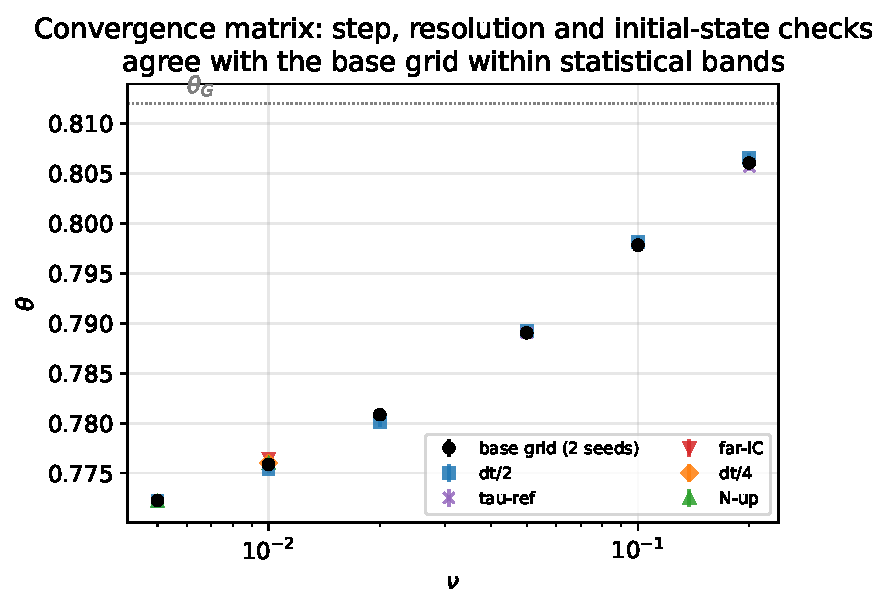
\includegraphics[width=0.66\textwidth]{theta_convergence.pdf}
\caption{The convergence matrix of Table~\ref{tab:convergence} plotted against the base
grid: time-step halving/quartering, spatial resolution $N=384$, and an independent
far-from-band initial condition all reproduce $\theta(\nu)$ within the conditional
statistical bands. Data: \texttt{anc/p2\_convergence\_v18.jsonl} and the tagged
receipt rows ($N{=}384$; $dt/2$ at $\nu=0.01$) of \texttt{p2\_results\_v18.jsonl}.}
\label{fig:convergence}
\end{figure}

\paragraph{Algebra --- symbolic layer (exact, zero polynomials over $\mathbb{Q}[a]$):}
\begin{itemize}
\item \texttt{anc/certify\_identities\_symbolic.py}:
  the five load-bearing identities --- (1) the $a$-cancellation $\langle N[\omega],\omega\rangle =
  (1+a/2)\int(H\omega)\omega^2$, (2) the first variation $D\mathcal{P}_1$ against an
  independent symbolic field, (3) the five-term inertial closed form $I(a)$,
  (4) Injection Lemma with symbolic per-mode rates $q_j$, (5) the A2 secondary term ---
  are each expanded to the \textbf{zero polynomial} in the symbolic mode
  coefficients $\{a_k, b_k\}$ (advection parameter $a$ symbolic), for all fields
  band-limited to $K \le 8$. This is a proof over $\mathbb{Q}[a]$ for those bands,
  not a floating-point check; Appendix~\ref{app:identities} proves each identity
  analytically for general fields, making this layer an independent verification
  rather than the carrier of the result.
\end{itemize}

\paragraph{Algebra --- spectral layer (band-limited, machine precision, independent code path):}
\begin{itemize}
\item Solver \texttt{anc/validate.py}: 12/12 ($u_x=H\omega$ $8\cdot10^{-17}$; $a=-2$ cancellation
  $4.5\cdot10^{-17}$; enstrophy-balance ratio 1.006; $d\mathcal{P}/dt$ chain-rule vs FD $8\cdot10^{-9}$).
\item Flux-law layer \texttt{anc/certify\_flux\_law.py}: L0/L1 decompositions, 5 seeds, $\le10^{-14}$
  ($a=-2$ cancellations to $10^{-19}$).
\item Production-balance inertial layer \texttt{anc/certify\_palinstrophy\_mine.py}: $D\mathcal{P}_1$ and $I(a)$, 4 seeds,
  machine precision (independently re-derived on separately written code).
\item Injection \texttt{anc/certify\_ito\_vanishing.py}: homogeneous It\^o trace $10^{-16}$,
  anisotropic $\ne0$.
\item Projected generator \texttt{anc/certify\_projected\_generator.py}: the decomposition
  $I = I_M + R_M$; the support lemma ($R_M = 0$ for fields with $2K \le M$, exact zero) and its
  sharpness ($R_M \ne 0$ for $M < 2K$); the $M{=}1$ example of Remark~\ref{rem:m1} to machine
  precision against the exact rationals $I = \tfrac{15\pi}{4}A^4$, $W_1 = \tfrac{9\pi}{2}A^4$,
  $I_M = \mathcal{C}_1 = 0$.
\item Exact Gaussian constant \texttt{anc/certify\_theta\_G\_exact.py}: the five
  Wick sums in rational arithmetic, $\theta_G(\text{band}[1,4]) = 2017/2484$;
  scale-invariance and reality checks pass; MC cross-check through the independent
  solver-side code path to $5.6\cdot10^{-5}$; the exact rational is independently
  re-derived by pointwise Wick moments in Appendix~\ref{app:thmF}.
\end{itemize}

\paragraph{Measurement (dynamical solver at stationarity; the \S4 stationary campaign unless noted):}
\begin{itemize}
\item (L0) $\nu E[\int\omega_x^2]/(\tfrac12 B_0) \in [0.977, 1.030]$ (seed-pooled per $\nu$; per-seed $[0.95, 1.06]$) across $\nu \in [0.005, 0.2]$ (uniform).
\item Anomalous cascade $E[\mathcal{E}_1] \sim \nu^{-1.002}$, $R^2=0.9999$, prefactor $0.0400$ vs $B_0/4 = 0.0400$.
\item $(\mathrm{FL}\infty)$ broad flux maximum (not a resolved plateau), through the Theorem A1 identity $\Pi(K) = \tfrac12 B_0 - \rho_\nu(\{|k|<K\})$ ($K>k_f$): $\Pi/(\tfrac12 B_0) = 0.872, 0.834, 0.757, 0.600$ at $K = 5, 6, 8, 12$, $\nu=0.005$ (maximum approaching 1 as $\nu\to0$; $<$1 octave of scale separation).
\item $a$-monotonicity: $E[\mathcal{P}_1]$ rises monotonically ($\approx3\times$) over $a: -2\to-0.5$, blow-up at $a=0$ (exploratory sweep; qualitative, no error bars quoted).
\item Large-$\nu$ limit (exact-OU stepping): $\theta_G(\text{band}) = 0.8119\pm10^{-4}$
  (Gaussian sampling, $N_{\rm MC}=2\cdot10^5$); SDE grid $\nu\in\{0.5,1,2,5,10,20\}\times2$ seeds,
  all $\theta\in[0.8107,0.8126]$ including CI95 half-widths (point estimates
  $0.8111$--$0.8123$; block-bootstrap CI95, split-half $z$ clean,
  $dt/5$-stable); balance closure at $\nu=2$: $E[I]=1.1124\cdot10^{-3}\pm8\cdot10^{-6}$
  vs $-\nu E[Y]=1.1730\cdot10^{-3}\pm1.1\cdot10^{-4}$, $z(\mathrm{diff})=-0.54$
  (\texttt{anc/theta\_large\_nu\_exact\_ou.log}, \texttt{anc/closure\_balance\_check.log}).
\item Stationary campaign (\S4 table; \texttt{anc/p2\_campaign\_v18.py}
  + \texttt{p2\_results\_v18.jsonl} + \texttt{p2\_analysis.py}): 6 $\nu$-points
  $\times$ 2 seeds, split-half $\max|z| = 1.7$ (all $<2$) on $I, W_1,
  \mathcal{E}_1, D$; deficit log-law, $\rho_\nu$ rates, $(\star)$ refutation, and
  the moment-form Cor E inputs ($E[Y^2]$, negative inertial-generation fraction $0$) all from the
  same runs.
\item Convergence matrix (Table~\ref{tab:convergence};
  \texttt{anc/p2\_convergence\_matrix.py (driven on the projected solver)} + \texttt{p2\_convergence\_v18.jsonl}): $dt/2$ at
  every campaign $\nu$, $dt/4$ at $\nu=0.01$, $N=384$ at $\nu \in \{0.01, 0.005\}$,
  an independent far-from-band initial condition, and $\tau_{\rm int}$ for $I$, $W_1$,
  $\theta$ --- all consistent with the base grid.
\item \emph{The coarse exploratory sweep (stationarity-$z$ 13--28; $\nu=0.02$
  under-resolved; 3-seed ensembles) is retained only for the qualitative $a$-dependence;
  every quantitative flux/scaling number above is from the stationary campaign.}
\end{itemize}

\paragraph{Cross-validation (independent implementations):} the inertial formula
$I(a)$ is certified
independently in \texttt{anc/certify\_palinstrophy\_mine.py} and by a separate,
independently-coded three-derivation of $D\mathcal{P}_1$ from the solver primitives
(each written blind to the other); the
two agree to machine precision.



\section{Proof of Theorem~F (large-$\nu$ limit of the diagnostic, Galerkin level)}
\label{app:thmF}

Fix the Galerkin cutoff $M \ge k_f$ and work on $E_M = P_M L^2_0(\mathbb{T})$ (real, mean-zero, modes
$1 \le |k| \le M$), with
\begin{equation}
  d\omega = \bigl(N_M[\omega] + \nu\omega_{xx}\bigr)\,dt + dW, \qquad N_M[\omega] = P_M N[P_M\omega],
\end{equation}
$N[\omega] = -au\omega_x + v\omega$ at $a=-2$, homogeneous band noise $b_k = f(|k|)$ on
$1 \le |k| \le k_f \le M$, and $B_0 = \sum_k b_k^2 = \mathrm{Tr}\,Q > 0$. Write $V(\omega) = \|\omega\|_{L^2}^2$
and $s^2 = B_0/(2\nu)$. On the finite-dimensional $E_M$ all Sobolev norms are equivalent (constants
depending on $M$), and $I$, $W_1$ and the Poisson potentials below are polynomials of degree $\le 5$
in the mode coordinates. The It\^o generator splits as $\mathcal{L} = \mathcal{L}_0 + \mathcal{L}_1$,
with $\mathcal{L}_0 F = \langle\nu\omega_{xx},DF\rangle + \tfrac12\mathrm{Tr}(QD^2F)$ (the
Ornstein--Uhlenbeck part) and
$\mathcal{L}_1 F = \langle N_M[\omega],DF\rangle$.

\emph{The Gaussian reference measure, explicitly.} The stationary law of $\mathcal{L}_0$ is the
\textbf{degenerate} Gaussian
\begin{equation}
\begin{aligned}
  G_\nu \;=\; \mathcal{N}\Bigl(0,\ \mathrm{diag}\bigl(b_k^2/(2\nu k^2)\bigr)\Bigr)
  \ &\text{on the forced band } 1 \le |k| \le k_f \\
  {}\otimes\ \delta_0 \ &\text{on the unforced modes } k_f < |k| \le M:
\end{aligned}
\end{equation}
the OU drift $-\nu k^2$ damps every mode, but noise enters only the band, so the unforced
modes relax to zero under $\mathcal{L}_0$. All Wick sums below therefore range over the
band modes only (this is why $\theta_G$ is a functional of the forcing \emph{shape}). Note
the invariant measures $\mu_\nu$ of the full \emph{nonlinear} system are not supported on
the band: $\mathcal{L}_1$ transfers mass to all modes $\le M$; only the reference Gaussian
is degenerate.

\emph{Norms.} For a polynomial $F = \sum_\alpha c_\alpha\, x^\alpha$ in the mode
coordinates $\{x_k\}$ of $E_M$, write $\|F\|_{\mathrm{coeff}} \eqdef \max_\alpha |c_\alpha|$
(maximal coefficient magnitude in the monomial basis); this is the norm used for the
coefficient bounds below. Throughout, $\theta_G = E_{G_\nu}[I]/E_{G_\nu}[W_1]$,
which is $\nu$-independent (both quartic, the rescaled shape $\nu$-independent).

\begin{lemma}[Hereditary cancellation]\label{lem:appfact0}
$\langle N_M[\omega],\omega\rangle = 0$ for every $\omega \in E_M$.
\end{lemma}

\emph{Proof.} As $\omega \in E_M$ is band-limited to $|k|\le M$, the idempotent $P_M$ is self-adjoint
and fixes $\omega$, so $\langle N_M[\omega],\omega\rangle = \langle N[\omega],\omega\rangle
= (1+a/2)\int(H\omega)\omega^2 = 0$ at $a=-2$ (Theorem~A0). $\qed$

\begin{lemma}[Moment bounds]\label{lem:appmoments}
For every $p \ge 1$ and every invariant measure $\mu_\nu$ of the Galerkin system,
$E_{\mu_\nu}[V^p] \le (2p-1)!!\,(B_0/2\nu)^p = (2p-1)!!\,s^{2p}$; consequently $E_{\mu_\nu}[\mathcal{L}F]=0$
for every polynomial $F$.
\end{lemma}

\emph{Proof.} By Lemma~\ref{lem:appfact0}, $\mathcal{L}V = -2\nu\|\omega_x\|^2 + B_0 \le -2\nu V + B_0$
(Poincar\'e $\|\omega_x\|^2 \ge \|\omega\|^2$ on mean-zero modes; the It\^o trace is $B_0$), and the
carr\'e du champ satisfies $\Gamma(V) = 4\sum_{k\in\text{band}}b_k^2|\hat\omega_k|^2 \le 4B_0 V$. Hence
\begin{equation}
  \mathcal{L}V^p = pV^{p-1}\mathcal{L}V + \tfrac12 p(p-1)V^{p-2}\Gamma(V) \le -2p\nu V^p + p(2p-1)B_0 V^{p-1}.
\end{equation}
To use $E_\mu[\mathcal{L}(\cdot)]=0$ before finiteness of moments is known, apply the generator to
concave cutoffs $\chi_R(V^p)$ ($\chi_R$ smooth, concave, $\chi_R(t)=t$ for $t\le R$,
$\chi_R'\in[0,1]$, $\chi_R''\le0$, $\chi_R\uparrow\mathrm{id}$): then $\mathcal{L}\chi_R(V^p)
= \chi_R'\,\mathcal{L}V^p + \tfrac12\chi_R''\,\Gamma(V^p) \le \chi_R'\,\mathcal{L}V^p$
($\Gamma \ge 0$, $\chi_R'' \le 0$), and
$\chi_R(V^p)$ is bounded with bounded derivatives, so $E_\mu[\mathcal{L}\chi_R(V^p)] = 0$ for every
invariant $\mu$. Proceed by induction on $p$ (base $E_\mu[V^0] = 1$), assuming
$E_\mu[V^{p-1}] < \infty$. Combining the two displays,
\begin{equation*}
\begin{aligned}
  0 &\;\le\; E_\mu\bigl[\chi_R'(V^p)\bigl(-2p\nu V^p + p(2p-1)B_0 V^{p-1}\bigr)\bigr],\\
  \text{i.e.}\qquad
  2p\nu\, E_\mu[\chi_R'(V^p)\,V^p] &\;\le\; p(2p-1)B_0\, E_\mu[\chi_R'(V^p)\,V^{p-1}],
\end{aligned}
\end{equation*}
where the right side is $\le p(2p-1)B_0\,E_\mu[V^{p-1}] < \infty$ ($0 \le \chi_R' \le 1$,
$V \ge 0$) --- note both integrands are nonnegative, so no sign-splitting is needed. As
$R\uparrow\infty$, $\chi_R'(V^p)\,V^p \to V^p$ pointwise, and Fatou's lemma gives
$2p\nu\,E_\mu[V^p] \le p(2p-1)B_0\,E_\mu[V^{p-1}]$ --- in particular $E_\mu[V^p] < \infty$
--- i.e.\ $E_\mu[V^p] \le (2p-1)(B_0/2\nu)\,E_\mu[V^{p-1}]$, and the induction yields the
bound. With all moments finite, dominated localization gives $E_\mu[\mathcal{L}F] = 0$ for
every polynomial $F$, using neither uniqueness nor ergodicity. $\qed$

For a polynomial $P$ homogeneous of degree $d$, the bound and H\"older give $E_{\mu_\nu}|P| \le C(P,M)\,s^d$.

\begin{lemma}[Poisson equation on polynomials]\label{lem:apppoisson}
For every polynomial $F$ of degree $d$ with $E_{G_\nu}[F] = 0$ there is a polynomial
$\varphi_F$ of the same degree
with $\mathcal{L}_0\varphi_F = F$ and, writing $\varphi_F = \sum_q \varphi_F^{(q)}$ for
its degree-$q$ homogeneous parts, the coefficient bounds
$\|\varphi_F^{(q)}\|_{\mathrm{coeff}} \le C(F,M)\,\nu^{-1}\max\!\bigl(1,(B_0/\nu)^{(d-q)/2}\bigr)$,
where $C(F,M)$ depends only on $\|F\|_{\mathrm{coeff}}$, $d$, and the number of modes.
\end{lemma}

\emph{Proof.} In mode coordinates $\mathcal{L}_0 = D + T$, where $D = -\sum_k\gamma_k x_k\partial_{x_k}$
($\gamma_k = \nu k^2$) is diagonal on monomials with eigenvalue $-\sum_k\alpha_k\gamma_k \le -\nu$ on
every non-constant monomial (since $\sum_k\alpha_k k^2 \ge 1$) and kills constants, and
$T = \tfrac12\sum_{k\in\text{band}}q_k\partial^2_{x_k}$ lowers degree by two ($q_k \le B_0$). Let
$\Pi_0$ be the projection onto the constant monomial and define $D^{-1}$ \emph{on
$\mathrm{Ran}(1-\Pi_0)$ only}, where $D$ is invertible with $\|D^{-1}\| \le \nu^{-1}$
(a centered polynomial can carry a nonzero constant \emph{monomial} even though its
Gaussian mean vanishes, so this restriction is not vacuous). Set
$\varphi_F = \sum_{j\ge0}\bigl(-D^{-1}(1-\Pi_0)T\bigr)^{j}D^{-1}(1-\Pi_0)F$
(a finite sum, $j \le d/2$, since $T$ lowers degree): dropping the constant component at
each stage yields $\mathcal{L}_0\varphi_F = F + c$ for some constant $c$. Taking
$E_{G_\nu}$ of both sides: $E_{G_\nu}[\mathcal{L}_0\varphi_F] = 0$ ($G_\nu$ is the
stationary law of $\mathcal{L}_0$) and $E_{G_\nu}[F] = 0$, so $c = 0$. Each $D^{-1}$
contributes a factor $\le\nu^{-1}$, each $T$ a factor $\le B_0$. $\qed$

\begin{lemma}[Correction identity]\label{lem:appcorr}
For every polynomial $F$ and every invariant $\mu_\nu$, with $\tilde F = F - E_{G_\nu}[F]$,
\begin{equation}
  E_{\mu_\nu}[F] - E_{G_\nu}[F] = -\,E_{\mu_\nu}\!\bigl[\langle N_M[\omega], D\varphi_{\tilde F}\rangle\bigr].
\end{equation}
\end{lemma}

\emph{Proof.} $0 = E_\mu[\mathcal{L}\varphi_{\tilde F}] = E_\mu[\mathcal{L}_0\varphi_{\tilde F}]
+ E_\mu[\mathcal{L}_1\varphi_{\tilde F}] = E_\mu[\tilde F] + E_\mu[\langle N_M,D\varphi_{\tilde F}\rangle]$,
the generator identity for the polynomial $\varphi_{\tilde F}$ being justified by
Lemma~\ref{lem:appmoments}. $\qed$

\begin{lemma}[Galerkin-defect bound]\label{lem:apprm}
Let $M \ge 2k_f$. Then $E_{G_\nu}[R_M] = 0$, and for every invariant measure $\mu_\nu$
of the Galerkin system, $|E_{\mu_\nu}[R_M]| \le C(M)\,\nu^{-1}s^5$.
\end{lemma}

\emph{Proof.} $G_\nu$ is supported on the forced band $|k| \le k_f$ (the degenerate
Gaussian above), and on band-supported fields $R_M$ vanishes pointwise by
Lemma~\ref{lem:rm} (its two factors are quadratic, hence supported on modes
$\le 2k_f \le M$, which $Q_M$ annihilates); so $E_{G_\nu}[R_M] = 0$. Since $R_M$ is a
quartic polynomial in the mode coordinates of $E_M$, Lemma~\ref{lem:appcorr} with the
coefficient bounds of Lemma~\ref{lem:apppoisson} gives the quintic bound
$|E_{\mu_\nu}[R_M] - E_{G_\nu}[R_M]| \le C(M)\,\nu^{-1}s^5$, exactly as for
$F \in \{I, W_1\}$ in the assembly below. $\qed$

\emph{Proof of Theorem~F.} Apply Lemma~\ref{lem:appcorr} to $F \in \{I, W_1\}$ (quartic, $d=4$). The
integrand $\langle N_M[\omega], D\varphi_{\tilde F}\rangle$ is a polynomial whose degree-$(5-2j)$ part
carries coefficients $\le C(M,F)\,B_0^j\nu^{-j-1}$ in $\|\cdot\|_{\mathrm{coeff}}$
(Lemma~\ref{lem:apppoisson}; $N_M$ is quadratic
with $M$-bounded coefficient tensors). Here and below, $C(M,F)$ aggregates three
$M$-dependent quantities: the number of monomials of the quartic $F$ (at most
$O(M^4)$), $\max_{k,l}$ of the quadratic-form coefficients of $N_M$ (polynomial in $M$
through the $u$, $v$, $\partial_x$ multipliers on modes $\le M$), and the length
$\le d/2 + 1$ of the nilpotent series in Lemma~\ref{lem:apppoisson} --- this is the sole
source of the $M$-growth of the constant in Theorem~F. By the consequence of Lemma~\ref{lem:appmoments} and
$s^2 = B_0/2\nu$,
\begin{equation}
  |E_\mu[F] - E_G[F]| \;\le\; \sum_{j=0}^{2} C\,B_0^j\,\nu^{-j-1}\,s^{5-2j}
  \;=\; C\,\nu^{-1}s^5\sum_{j=0}^{2}\Bigl(\tfrac{B_0}{\nu s^2}\Bigr)^{\!j} \;=\; C'\,\nu^{-1}s^5,
\end{equation}
the sum being finite ($B_0/(\nu s^2) = 2$ and $j$ ranges over $\{0,1,2\}$). Both Gaussian means are
exactly quartic, $E_G[W_1] = c_W s^4$ and $E_G[I] = c_I s^4$ with $c_W > 0$ (as $W_1 \ge 0$ and
$E_G[W_1] = 0$ only if $v\omega_x \equiv 0$ $G$-a.s., impossible for a non-degenerate band Gaussian).
Hence, for $\nu \ge \nu_0$ so that $E_\mu[W_1] \ge c_W s^4/2$,
\begin{equation}
  |\theta(\mu_\nu) - \theta_G| = \frac{|E_\mu I\cdot E_G W_1 - E_G I\cdot E_\mu W_1|}{E_\mu W_1\cdot E_G W_1}
  \;\le\; \frac{C\,(\nu^{-1}s^5)\,s^4}{s^8} \;=\; C\,\frac{s}{\nu} \;=\; C\sqrt{B_0/2}\;\nu^{-3/2}.
\end{equation}
For the balance coefficient at $M \ge 2k_f$: by Lemma~\ref{lem:apprm} and
$E_\mu[W_1] \ge c_W s^4/2$,
\begin{equation}
  |\theta_M(\mu_\nu) - \theta(\mu_\nu)| = \frac{|E_\mu[R_M]|}{E_\mu[W_1]}
  \le \frac{C\,\nu^{-1}s^5}{c_W s^4/2} = C'\sqrt{B_0/2}\;\nu^{-3/2},
\end{equation}
and the $\theta_M$ bound follows by the triangle inequality; since
$\theta_G \ge \theta_{G,\min} > 0$ (Lemma~\ref{lem:appthetaG}),
$\mathcal{C}_1 = -\theta_M(\mu_\nu)\,E_\mu[W_1] < 0$ for all $\nu \ge \nu_1(M, B_0, \text{shape})$.
$\qed$

\begin{lemma}[Positivity of the Gaussian limit]\label{lem:appthetaG}
For homogeneous band noise with arbitrary amplitudes $b_k \ge 0$ (not all zero) on
$1 \le |k| \le k_f$,
\begin{equation*}
  \theta_G \;=\; \frac{E_G[I]}{E_G[W_1]} \;\ge\; \theta_{G,\min}
  \;=\; \frac13 + \frac{\sqrt{69}}{18} \;>\; 0 .
\end{equation*}
\end{lemma}

\emph{Proof.} Wick's theorem over the band Gaussian (per-pair variances $s_k^2$) gives
\begin{equation*}
  E_G[W_1] = \sum_{k} 36\pi k^2 s_k^4
  + \sum_{i<j} 12\pi\,(i^2 + 4ij + j^2)\, s_i^2 s_j^2,
\end{equation*}
a direct two-mode computation (the weights of the modes actually forced are strictly
positive, while zero-amplitude modes contribute zero-weight terms that drop from the
sums; at least one positive term survives since not all $b_k$ vanish, so
$E_G[W_1] > 0$), and correspondingly
$E_G[I] = \sum_k \tfrac56\cdot 36\pi k^2 s_k^4 + \sum_{i<j} \theta_G(j/i)\cdot
12\pi(i^2+4ij+j^2)\, s_i^2 s_j^2$, where $\tfrac56$ is the certified diagonal
self-ratio and $\theta_G(m) = (5+7m+3m^2)/(3+12m+3m^2)$ the certified pairwise ratio
(\S4). Every ratio appearing is $\ge \min\bigl(\tfrac56,\ \min_{m>1}\theta_G(m)\bigr)
= \theta_{G,\min}$ (interior minimum at $m^* = (2+\sqrt{69})/5$, \S4). For positive
weights $\beta_\alpha > 0$ and ratios $r_\alpha \ge r$, the weighted mediant satisfies
$\sum_\alpha \beta_\alpha r_\alpha / \sum_\alpha \beta_\alpha \ge r$; apply it with
$\beta$ = the displayed $W_1$-weights times the variance monomials. $\qed$

\emph{The exact constant.} For the flat band $[1,4]$ ($\sigma_k^2 \propto 1/k^2$) the five Wick sums
evaluate in exact rational arithmetic (\texttt{anc/certify\_theta\_G\_exact.py}, Monte-Carlo
cross-checked through the independent solver-side code path to $5.6\cdot10^{-5}$) to $T_1 = 115/2$,
$T_2 = T_3 = T_5 = -625/36$, $T_4 = -395/36$ (in units $2\pi\cdot\text{scale}^2$, with per-pair
variances $s_k^2 = \text{scale}^2/k^2$ and $\text{scale}^2 = 2$ for the tabulated values; only the
final ratio is normalization-independent), giving
$E_G[I] = (10085/36)\cdot 2\pi$, $E_G[W_1] = 345\cdot 2\pi$, and
\begin{equation}
  \theta_G(\text{band}\,[1,4]) = \frac{10085/36}{345} = \frac{2017}{2484} = 0.811996779\ldots
\end{equation}
A pointwise-moment cross-derivation of $T_1$: by Gaussian factorization
$E_G[T_1]/2\pi = E[v^2]\,E[\omega_x^2] + 2\,E[v\omega_x]^2 = (205/72)\cdot 8 + 2(25/6)^2 = 115/2$; the
coincidence $T_2 = T_3 = T_5 = -625/36$ is structural, and for $T_5$ the internal pairing vanishes on
$\mathrm{sgn}(0)=0$. The value $\theta_{G,\min} = 1/3 + \sqrt{69}/18 \approx 0.7948$
is the infimum of the \emph{cross-mode coefficient ratio} $\theta_G(m)$ --- a universal lower bound,
not an attained full-shape minimum; the band value sits strictly above it, being the $c_W$-weighted mediant
of the diagonal self-ratio $5/6$ and the cross ratios, all $\ge \theta_{G,\min}$ with positive
weights.

\emph{Honest scope.} The constant $C = C(M)$ grows with the cutoff (through the norm-equivalence
constants and the coefficient tensors of $N_M$); removing it needs uniform-in-$M$ moment bounds in a
norm strong enough for the quintic error together with Galerkin convergence of invariant measures ---
both open. The small-$\nu$ regime is untouched.

\section{Proofs of the algebraic identities (general fields)}
\label{app:identities}

This appendix proves every load-bearing algebraic identity of \S3--\S4 for general
smooth mean-zero fields on $\mathbb{T}$ --- in particular for trigonometric polynomials
of \emph{arbitrary} band --- so the symbolic $K \le 8$ certificates of Appendix~\ref{app:verification} are an
independent verification layer, not the carrier of the results. We use three standard
properties of the Hilbert transform on mean-zero fields:
\begin{itemize}
\item[(H1)] skew-adjointness: $\int (Hf)\,g = -\int f\,(Hg)$;
\item[(H2)] commutation with derivatives: $H\partial_x = \partial_x H$ (both are Fourier
multipliers); in particular $v_x = H\omega_x$ for $v = H\omega$;
\item[(H3)] $u = -\Lambda^{-1}\omega$, so $u_x = H\omega = v$.
\end{itemize}
Every identity below is an exact integral identity in the field; each is bilinear or
multilinear in $\omega$, so it holds identically for $\omega \in E_M$ at any Galerkin cutoff
$M$ (where needed, $P_M$ is self-adjoint and fixes its range, so
$\langle P_M N[P_M\omega], g\rangle = \langle N[\omega], P_M g\rangle = \langle N[\omega], g\rangle$
\textbf{for band-limited} $g \in E_M$). \emph{This caveat is load-bearing:} in the
stationarity balances the role of $g$ is played by the test function $DF$, which is
band-limited for the \S3 balances ($g = \omega,\ P_{<K}\omega,\ \omega_{xx} \in E_M$)
but \textbf{not} for the production balance of \S4, whose gradient $D\mathcal{P}_1$ is
quadratic and leaves $E_M$ --- there the exact Galerkin statement uses the projected
pairing $I_M = \langle P_M N, P_M D\mathcal{P}_1\rangle$ with the defect $R_M$
(\S4, Lemma~\ref{lem:rm}). The generator identities $E_\mu[\mathcal{L}F] = 0$ invoked below
are theorems at any fixed Galerkin truncation (Lemma~\ref{lem:appmoments}), with the
gradient read as $P_M DF$, and formal for the untruncated SPDE (\S2 convention).

\subsection{The advective cancellation}

\begin{lemma}[Advective cancellation]\label{lem:cancel}
For every smooth mean-zero $\omega$ and every $a$,
\begin{equation}
  \langle N[\omega], \omega\rangle \;=\; \Bigl(1 + \frac a2\Bigr)\int (H\omega)\,\omega^2,
  \qquad N[\omega] = -a u\omega_x + v\omega .
\end{equation}
In particular $\langle N[\omega],\omega\rangle = 0$ at $a = -2$.
\end{lemma}

\emph{Proof.} $\langle v\omega, \omega\rangle = \int v\,\omega^2$. For the transport term,
integrate by parts using (H3):
\begin{equation}
  \langle -a u\omega_x, \omega\rangle = -a\int u\,\omega\,\omega_x
  = -\frac a2 \int u\,(\omega^2)_x = \frac a2 \int u_x\,\omega^2 = \frac a2 \int v\,\omega^2 .
\end{equation}
Adding the two terms gives the claim. $\qed$

\subsection{Stationarity balances: proofs of Theorems A0 and A1}

Fix $K$ and set $F_K(\omega) = \tfrac12\|P_{<K}\omega\|_{L^2}^2$. Then $DF_K = P_{<K}\omega$
and $D^2F_K = P_{<K}$, so
\begin{equation}
  \mathcal{L}F_K = \langle P_{<K}\omega,\, N[\omega]\rangle
  + \nu\,\langle P_{<K}\omega,\, \omega_{xx}\rangle
  + \tfrac12\,\mathrm{Tr}(Q P_{<K}) .
\end{equation}
Since $P_{<K}$ is a self-adjoint idempotent commuting with $\partial_x$:
$\langle P_{<K}\omega, N[\omega]\rangle = \langle P_{<K}\omega, P_{<K}N[\omega]\rangle = -\Pi(K)$
(the definition of the flux, \S2);
$\nu\langle P_{<K}\omega, \omega_{xx}\rangle = -\nu\|P_{<K}\omega_x\|^2$ (integration by
parts); and $\mathrm{Tr}(Q P_{<K}) = \sum_{|k|<K} b_k^2 = B_0^{<K}$ (the basis $\{e_k\}$
diagonalizes both $Q$ and $P_{<K}$). Taking $E_\mu[\mathcal{L}F_K] = 0$,
\begin{equation}
  E_\mu[\Pi(K)] = \tfrac12 B_0^{<K} - \nu\,E_\mu\|P_{<K}\omega_x\|^2 ,
\end{equation}
which is Theorem A1. Letting
$P_{<K} = \mathrm{Id}$ (i.e.\ $K$ beyond the cutoff, or $K\to\infty$), the flux term is
$\langle \omega, N[\omega]\rangle = 0$ at $a=-2$ by Lemma~\ref{lem:cancel}, and the identity becomes
$\nu E_\mu[\int\omega_x^2] = \tfrac12 B_0$ --- Theorem A0. $\qed$

\subsection{Proof of Theorem A2}

Apply the generator to the palinstrophy $\mathcal{E}_1 = \tfrac12\int\omega_x^2$:
$D\mathcal{E}_1 = -\omega_{xx}$ and $D^2\mathcal{E}_1(h,h) = \|h_x\|^2$, so
$\mathrm{Tr}(Q D^2\mathcal{E}_1) = \sum_k b_k^2\,\|(e_k)_x\|^2 = \sum_k b_k^2 k^2 = B_2$
(the $\{e_k\}$ are $L^2$-normalized). Hence $E_\mu[\mathcal{L}\mathcal{E}_1] = 0$ reads
\begin{equation}
  \nu\,E_\mu\Bigl[\int\omega_{xx}^2\Bigr]
  = -\,E_\mu\bigl[\langle\omega_{xx}, N[\omega]\rangle\bigr] + \tfrac12 B_2 .
\end{equation}
It remains to identify the nonlinear term. Using (H3) and integration by parts,
\begin{align}
  -\langle\omega_{xx}, N[\omega]\rangle
  &= a\int u\,\omega_x\omega_{xx} - \int v\,\omega\,\omega_{xx} \notag\\
  &= \frac a2\int u\,(\omega_x^2)_x + \int (v\omega)_x\,\omega_x
  = -\frac a2\int v\,\omega_x^2 + \int v_x\,\omega\,\omega_x + \int v\,\omega_x^2 \notag\\
  &= \Bigl(1 - \frac a2\Bigr)\int v\,\omega_x^2 + \int v_x\,\omega\,\omega_x .
\end{align}
At $a = -2$ this is $2\int(H\omega)\omega_x^2 + \int(H\omega_x)\,\omega\,\omega_x = \Pi_1$. For the
secondary term, by (H2) and integration by parts,
\begin{equation}
  \int (H\omega_x)\,\omega\,\omega_x = \frac12\int (H\omega_x)\,(\omega^2)_x
  = -\frac12\int (H\omega_x)_x\,\omega^2 = -\frac12\int (H\omega_{xx})\,\omega^2 . \qquad\qed
\end{equation}

\subsection{The first variation of $\mathcal{P}_1$}

\begin{lemma}[First variation]\label{lem:dp1}
For $\mathcal{P}_1(\omega) = \int (H\omega)\,\omega_x^2$,
\begin{equation}
  D\mathcal{P}_1 = -H(\omega_x^2) - 2\,(H\omega_x)\,\omega_x - 2\,(H\omega)\,\omega_{xx} .
\end{equation}
\end{lemma}

\emph{Proof.} For a smooth perturbation $h$,
\begin{equation}
  \frac{d}{d\varepsilon}\Big|_{\varepsilon=0}\mathcal{P}_1(\omega + \varepsilon h)
  = \int (Hh)\,\omega_x^2 + 2\int (H\omega)\,\omega_x\, h_x .
\end{equation}
By (H1) the first term is $-\int h\,H(\omega_x^2)$. Integrating the second by parts and
using (H2),
\begin{equation}
  2\int (H\omega)\,\omega_x\, h_x = -2\int \bigl((H\omega)\,\omega_x\bigr)_x h
  = -2\int (H\omega_x)\,\omega_x\, h - 2\int (H\omega)\,\omega_{xx}\, h .
\end{equation}
Collecting the kernels gives the displayed $D\mathcal{P}_1$. $\qed$

\subsection{The inertial closed form $I(a)$ and the $W_1$--$N_1$ split}

\begin{proposition}[Inertial closed form]\label{prop:Ia}
With $b_{nl} = -a u\omega_x + v\omega$ and $D\mathcal{P}_1$ as in Lemma~\ref{lem:dp1},
\begin{equation}
\begin{aligned}
   I(a) \eqdef \langle b_{nl}, D\mathcal{P}_1\rangle
   = {}& (2-2a)\int v^2\omega_x^2 - 2a\int uv\,\omega_x\omega_{xx} + 2\int v v_x\,\omega\omega_x \\
   & + a\int u\,\omega_x\, H(\omega_x^2) - \int v\,\omega\, H(\omega_x^2) .
\end{aligned}
\end{equation}
At $a = -2$,
\begin{equation}
  I(-2) = \underbrace{6\int v^2\omega_x^2}_{=\,W_1} + 4\int uv\,\omega_x\omega_{xx}
  + 2\int v v_x\,\omega\omega_x - 2\int u\,\omega_x H(\omega_x^2) - \int v\,\omega\, H(\omega_x^2),
\end{equation}
so the nonlocal term in the split $I = W_1 - N_1$ is, explicitly,
\begin{equation}
  N_1 = -\,4\int uv\,\omega_x\omega_{xx} - 2\int v v_x\,\omega\omega_x
  + 2\int u\,\omega_x H(\omega_x^2) + \int v\,\omega\, H(\omega_x^2) .
\end{equation}
\end{proposition}

\emph{Proof.} Expanding $\langle -a u\omega_x + v\omega,\, D\mathcal{P}_1\rangle$ into the six
pairings (using $v_x = H\omega_x$, (H2)):
\begin{equation}
\begin{aligned}
  \langle v\omega, D\mathcal{P}_1\rangle
  &= -\int v\omega\,H(\omega_x^2) - 2\int v v_x\,\omega\omega_x - 2\int v^2\,\omega\omega_{xx},\\
  \langle -a u\omega_x, D\mathcal{P}_1\rangle
  &= a\int u\,\omega_x H(\omega_x^2) + 2a\int u v_x\,\omega_x^2 + 2a\int uv\,\omega_x\omega_{xx} .
\end{aligned}
\end{equation}
Two integration-by-parts conversions bring this to the displayed form:
\begin{itemize}
\item[(i)] $\displaystyle -2\int v^2\,\omega\omega_{xx} = 2\int (v^2\omega)_x\,\omega_x
  = 4\int v v_x\,\omega\omega_x + 2\int v^2\omega_x^2$;
\item[(ii)] $\displaystyle 0 = \int (u v\,\omega_x^2)_x
  = \int v^2\omega_x^2 + \int u v_x\,\omega_x^2 + 2\int uv\,\omega_x\omega_{xx}$
  \ (using $u_x = v$), whence
  $\int u v_x\,\omega_x^2 = -\int v^2\omega_x^2 - 2\int uv\,\omega_x\omega_{xx}$.
\end{itemize}
Substituting (i) and (ii),
\begin{equation}
  I(a) = (2-2a)\int v^2\omega_x^2 + 2\int v v_x\,\omega\omega_x - \int v\omega\,H(\omega_x^2)
  + a\int u\,\omega_x H(\omega_x^2) - 2a\int uv\,\omega_x\omega_{xx},
\end{equation}
which is the claim; the $a=-2$ specialization and the definition $N_1 \eqdef W_1 - I$
give the split. $\qed$

All five identities of this appendix are certified independently --- symbolically as
zero polynomials over $\mathbb{Q}[a]$ for bands $K \le 8$ and spectrally at machine
precision (Appendix~\ref{app:verification}); the derivations above remove the band restriction.

\begin{thebibliography}{9}

\bibitem{BCZPSW2020} J.~Bedrossian, M.~Coti Zelati, S.~Punshon-Smith, F.~Weber,
  \emph{Sufficient conditions for dual cascade flux laws in the stochastic 2d
  Navier--Stokes equations}, Arch. Ration. Mech. Anal. \textbf{237} (2020), no.~1,
  103--145. arXiv:1905.03299.

\bibitem{CHH2021} J.~Chen, T.~Y.~Hou, D.~Huang,
  \emph{On the finite time blowup of the De Gregorio model for the 3D Euler
  equations}, Comm. Pure Appl. Math. \textbf{74} (2021), no.~6, 1282--1350.
  arXiv:1905.06387.

\bibitem{CLM1985} P.~Constantin, P.~D.~Lax, A.~Majda,
  \emph{A simple one-dimensional model for the three-dimensional vorticity
  equation}, Comm. Pure Appl. Math. \textbf{38} (1985), no.~6, 715--724.

\bibitem{DeGregorio1990} S.~De Gregorio,
  \emph{On a one-dimensional model for the three-dimensional vorticity equation},
  J. Statist. Phys. \textbf{59} (1990), no.~5--6, 1251--1263.

\bibitem{Dudley2023} E.~Dudley,
  \emph{Necessary and sufficient conditions for Kolmogorov's flux laws on
  $\mathbb{T}^2$ and $\mathbb{T}^3$}, arXiv:2305.05717 (2023).

\bibitem{ElgindiJeong2020} T.~M.~Elgindi, I.-J.~Jeong,
  \emph{On the effects of advection and vortex stretching},
  Arch. Ration. Mech. Anal. \textbf{235} (2020), no.~3, 1763--1817.

\bibitem{FFS2026} S.~Fujita, R.~Fukuizumi, T.~Sakajo,
  \emph{Ergodicity for a Constantin--Lax--Majda--DeGregorio model of turbulent
  flow}, arXiv:2603.06182 (2026).

\bibitem{LiuLuWang2026} R.~Liu, K.~Lu, Z.~Wang,
  \emph{Mixed third-order flux laws for dual cascade in the stochastic SQG
  equation}, arXiv:2606.26788 (2026).

\bibitem{MS2016} T.~Matsumoto, T.~Sakajo,
  \emph{One-dimensional hydrodynamic model generating a turbulent cascade},
  Phys. Rev. E \textbf{93} (2016), 053101.

\bibitem{MS2017} T.~Matsumoto, T.~Sakajo,
  \emph{Turbulence, cascade and singularity in a generalization of the
  Constantin--Lax--Majda equation}, arXiv:1707.05205 (2017).

\bibitem{OSW2008} H.~Okamoto, T.~Sakajo, M.~Wunsch,
  \emph{On a generalization of the Constantin--Lax--Majda equation},
  Nonlinearity \textbf{21} (2008), no.~10, 2447--2461.

\bibitem{TS2023} Y.~Tsuji, T.~Sakajo,
  \emph{Statistical laws of a one-dimensional model of turbulent flows subject
  to an external random force}, Nonlinearity \textbf{36} (2023), no.~8, 4283--4302.
  doi:10.1088/1361-6544/acdfa3.

\end{thebibliography}

\end{document}
